\documentclass[a4paper,12pt]{article}
\usepackage{amsmath}
\usepackage{graphicx}
\usepackage{listings}
\usepackage{caption}
\usepackage{hyperref}
\usepackage{booktabs}
\usepackage{pgfplots} % For including plots
\usepackage{ragged2e}
\usepackage{listings}
\usepackage{float}
\usepackage{geometry}
\usepackage{wrapfig} % Required for wrapping text around figures
\geometry{margin=2.5cm} % <-- Set all margins to 2.5cm. Change as needed.
\usepackage[most]{tcolorbox}

\usepackage{graphicx} % For including images
\usepackage{caption}    % For customized captions
\usepackage{subcaption} % For subfigures (multiple images in one figure environment)
\usepackage{float}      % For more control over float placement, e.g., [H]
% Adjust geometry if needed for better page layout with many images
% \usepackage[margin=2.5cm]{geometry}


\hypersetup{
    hidelinks
}


\usepackage{xcolor}

\definecolor{codegreen}{rgb}{0,0.6,0}
\definecolor{codegray}{rgb}{0.5,0.5,0.5}
\definecolor{codepurple}{rgb}{0.58,0,0.82}
\definecolor{backcolour}{rgb}{0.95,0.95,0.92}

\tcbset{
    frame code={},
    center title,
    left=0pt,
    right=0pt,
    top=0pt,
    bottom=0pt,
    colback=backcolour,
    colframe=white,
    width=\dimexpr\textwidth\relax,
    enlarge left by=0mm,
    boxsep=5pt,
    arc=0pt,outer arc=0pt,
    }



\lstdefinestyle{mystyle}{
    backgroundcolor=\color{backcolour},   
    commentstyle=\color{codegreen},
    keywordstyle=\color{magenta},
    numberstyle=\tiny\color{codegray},
    stringstyle=\color{codepurple},
    basicstyle=\ttfamily\footnotesize,
    breakatwhitespace=false,         
    breaklines=true,                 
    captionpos=b,                    
    keepspaces=true,                 
    numbers=left,                    
    numbersep=5pt,                  
    showspaces=false,                
    showstringspaces=false,
    showtabs=false,                  
    tabsize=2
}

\lstset{style=mystyle}

\usepackage{graphicx} % Required for inserting images

\title{Human Computer Interaction}
\author{Budgify Report}
\date{Authors:\\ Onorio Iacobelli\\Alessandro Rocchi\\Alessandro Catalano}

\begin{document}

\maketitle

\tableofcontents

\section{Introduction}
Our idea was to create an application that would help users in managing their finances and set new goals. We didn't focus on a specific target audience as this is a topic relevant for all people, no matter age or job.

\section{Application scenario}
Budgify is a personal finance management application designed to assist users in effectively tracking their income and expenses, managing loans, and setting and achieving financial goals. The application is tailored for a broad user base, including students, professionals, and families, aiming to promote better financial awareness and discipline in everyday life.
\vspace{0.5cm}\\
In the current economic and technological context, individuals often struggle with fragmented or unclear financial habits. Budgify addresses this challenge by offering a unified platform to log transactions, monitor outstanding debts or credits, and visualize progress toward financial objectives, such as saving for a vacation or repaying a loan. The core motivation behind Budgify is to combine usability, motivation, and clarity to encourage users to maintain healthy financial habits over time.
\vspace{0.5cm}\\
\textbf{Constraints and Considerations:}
\begin{itemize}
    \item Organizational Constraints: As the project was developed in an academic context with a limited timeframe and team size, resource allocation and scope had to be carefully managed. Prioritization was essential to focus on the most impactful features.
    \item User-Centric Constraints: The app had to remain intuitive and accessible, especially for non-expert users. This shaped decisions related to UI simplicity, onboarding processes, and feature visibility.
    \item Platform Constraints: Budgify was developed as a native Android app, which influenced design decisions related to UI components, device compatibility, and data storage practices.
\end{itemize}

\section{Work Plan}

The development of Budgify followed an iterative, user-centered methodology that ensured continuous feedback and improvement across the development cycle. The process was structured into four main phases:
\subsection{Requirements Gathering}
The initial phase focused on understanding user needs and identifying key functionalities. This involved:
\begin{itemize}
    \item A questionnaire distributed to a wide audience to gather quantitative insights on users' financial management habits and expectations.
    \item Interviews with a smaller, representative group of potential users to gather qualitative feedback and user stories.
    \item Competitor analysis to study strengths and weaknesses of similar finance apps, identifying market gaps and opportunities for differentiation.
\end{itemize}
\subsection{Analysis and Design}
In this phase, the collected data was translated into:
\begin{itemize}
    \item Personas and usage scenarios, capturing various user types and their goals.
    \item A set of functional and non-functional requirements.
    \item The first prototype (Prototype 0), consisting of static mockups that helped validate navigation flows and feature prioritization before moving to implementation.
\end{itemize}
\subsection{Implementation and Prototyping}
The app was developed over three iterative prototypes:
\begin{itemize}
    \item \textbf{Prototype 0:} Static mockups created based on initial design ideas and user feedback from the requirements phase.
    \item \textbf{Prototype 1:} Two alternative interactive prototypes implemented with partial functionality. These were used for early usability testing and comparative evaluation to assess visual layout and user flow preferences.
    \item \textbf{Prototype 2:} Final working version of Budgify, refined based on insights from Prototype 1 evaluations. This version integrated core functionalities (transaction logging, loan management, goal tracking) and was tested for performance and user satisfaction.
\end{itemize}
\subsection{Evaluation and Conclusion}
The final phase focused on:
\begin{itemize}
    \item User evaluation of the final prototype through usability testing and surveys, measuring effectiveness, efficiency, and user satisfaction.
    \item Bug fixing and final refinements based on evaluation feedback.
    \item Documentation of the entire development process, including the rationale behind design choices, challenges encountered, and lessons learned.
\end{itemize}
This structured, feedback-driven approach ensured that Budgify evolved according to real user needs, resulting in a more robust and usable final product.
\section{Requirements Analysis}

\subsection{Personas and Scenarios}

\subsubsection{Alex Jameson – The Student with the Dream of a Car}
\begin{figure}[H]
    \centering
    
\includegraphics[scale=0.1]{alex.png}
\end{figure}
\begin{enumerate}
    \item Personality and Behavior:
    
    Alex is an ambitious and forward-thinking university student, constantly striving for independence. He's disciplined in his studies and works part-time, but struggles with self-control when it comes to impulsive spending. Deep down, Alex is motivated by the desire to prove to himself and others that he can achieve major life goals on his own. He values freedom and sees owning a car as a symbol of personal success and responsibility.
    
    \item Scenario:
    
    Alex dreams of buying his first car but feels overwhelmed trying to balance his school workload, part-time job, and unpredictable spending habits. When he starts using "Budgify", it becomes more than just a budgeting tool, it’s his personal financial coach.
    
    \item Impact of "Budgify":
    
    Goal-Oriented Mindset: Alex sets a specific savings goal in "Budgify" for his car, breaking it down into manageable monthly targets. Seeing his progress visually keeps him motivated and focused.
    
    Behavioral Awareness: With "Budgify" spending insights, Alex becomes more aware of his habitual takeout expenses. Recognizing the impact, he starts meal-prepping, not only saving money but also improving his health and self-discipline.
    
    Thanks to "Budgify", Alex gains a stronger sense of control and confidence in his financial decisions, ultimately purchasing his car without compromising his long-term security.

\end{enumerate}
\subsubsection{James Carter – The Man Who Got Fired}
\begin{figure}[H]
    \centering
    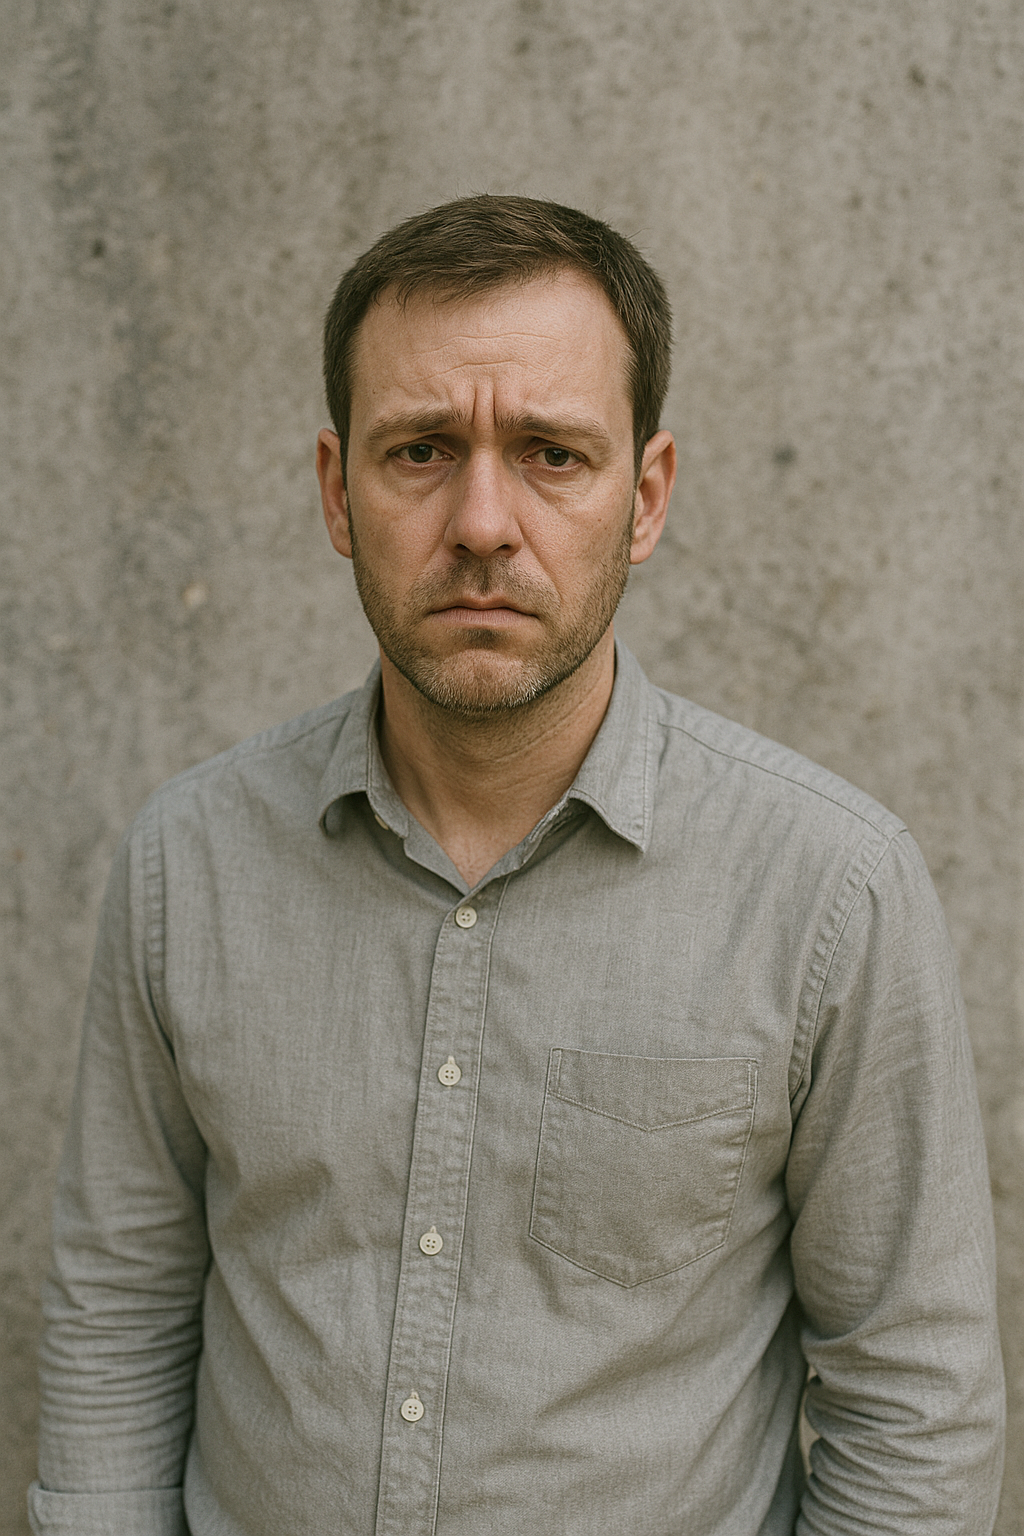
\includegraphics[scale=0.1]{james.png}
\end{figure}
\begin{enumerate}
    \item Personality and Behavior:
    
    James is a practical and resilient individual in his late 30s who thrives on stability. When he loses his job, his initial reaction is anxiety, bordering on hopelessness. Internally, he struggles with self-worth and the fear of losing control. However, James is also adaptive and willing to rebuild. He's detail-oriented and appreciates clarity when faced with uncertainty.
    
    \item Scenario:
    After being unexpectedly laid off, James feels lost and unsure of how long he can stay afloat. He turns to "Budgify" to regain a sense of direction and clarity during this uncertain time.
    
    \item Impact of "Budgify":
    
    Clarity in Chaos: "Budgify" helps James analyze his emergency fund and sets a realistic timeline for how long his current savings will last. This calms his anxiety and lets him focus strategically on his next steps.
    
    Structured Transition: As he begins freelancing, James uses "Budgify" to categorize different income sources, track tax-related expenses, and manage invoices. This organization helps him treat freelancing as a viable and structured career path.
    
    Thanks to "Budgify", James rebuilds his confidence and navigates unemployment with purpose, eventually stabilizing his finances and redefining his professional future.

\end{enumerate}
\subsubsection{Margaret "Maggie" Thompson – The Elder Who Wants to Go on a Cruise}
\begin{figure}[H]
    \centering
    
\includegraphics[scale=0.1]{margaret.png}
\end{figure}
\begin{enumerate}
    \item Personality and Behavior:
    
    Maggie is a lively, optimistic retiree with a zest for life. She’s careful with money but believes in enjoying the fruits of her lifelong labor. Internally, she’s driven by the need to feel independent and self-sufficient, even in her golden years. She's curious, enjoys planning, and takes pride in managing her finances herself rather than relying on her children.
    
    \item Scenario:
    
    With a long-anticipated cruise around the Mediterranean on the horizon, Maggie wants to enjoy herself without falling into careless spending. She downloads "Budgify" to help her prepare for the trip.
    
    \item Impact of "Budgify":
    
    Confident Planning: Maggie uses "Budgify" to create a personalized trip budget, dividing expenses into categories like travel, lodging, excursions, and on-board spending. The app gives her peace of mind by projecting her affordability.
    
    Conscious Spending: During the trip, "Budgify" tracks her spending in real time, sending gentle alerts when she’s nearing her limits. This empowers her to make informed choices—buying meaningful souvenirs while skipping unnecessary extras.
    
    Thanks to "Budgify", Maggie enjoys her cruise worry-free, proud of having full control over her finances, and returns home with wonderful memories—not debt.
\end{enumerate}
\subsection{User analysis}

\subsubsection{Questionnaire}
The questionnaire helped in better understanding our potential targeted users.
We reached 29 people and these data were useful to validate our assumptions and
ideas and to improve.
\begin{figure}[H]
    \centering
    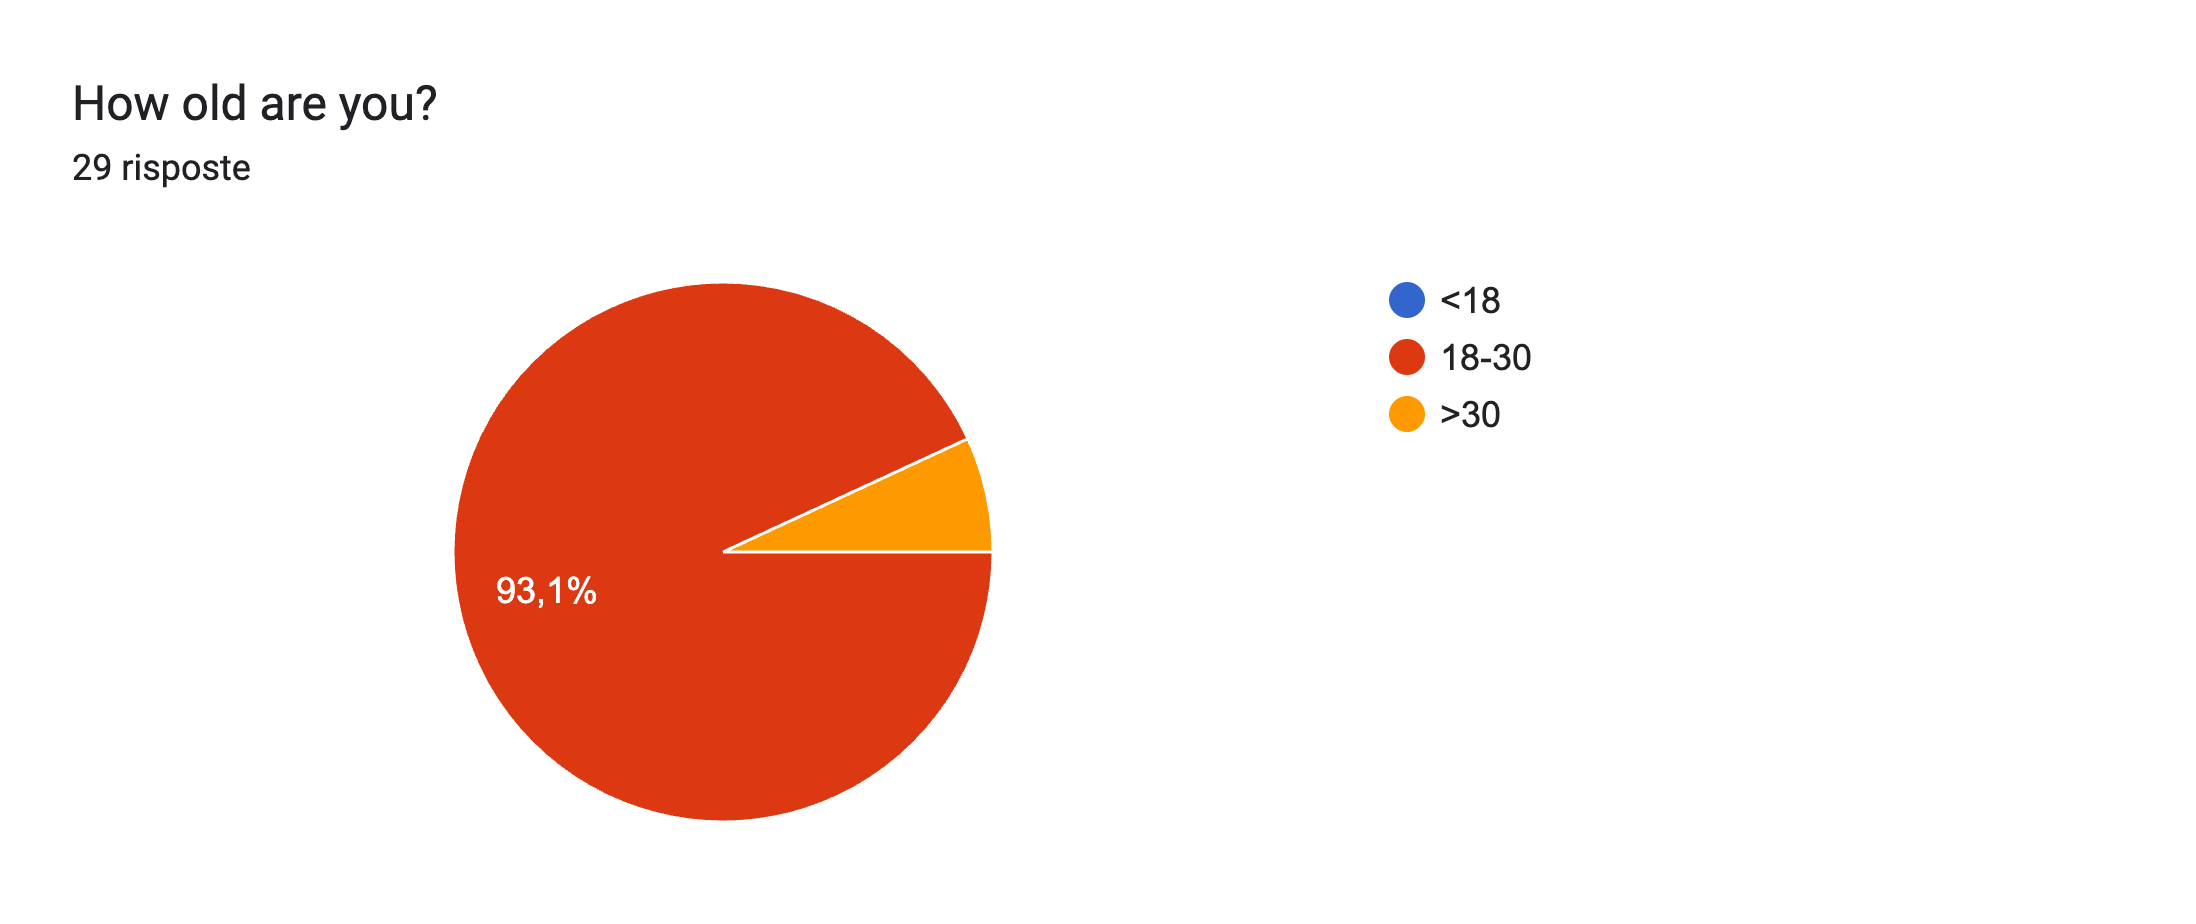
\includegraphics[width=\linewidth]{imagequest9.jpg}
\end{figure}

\begin{figure}[H]
    \centering
    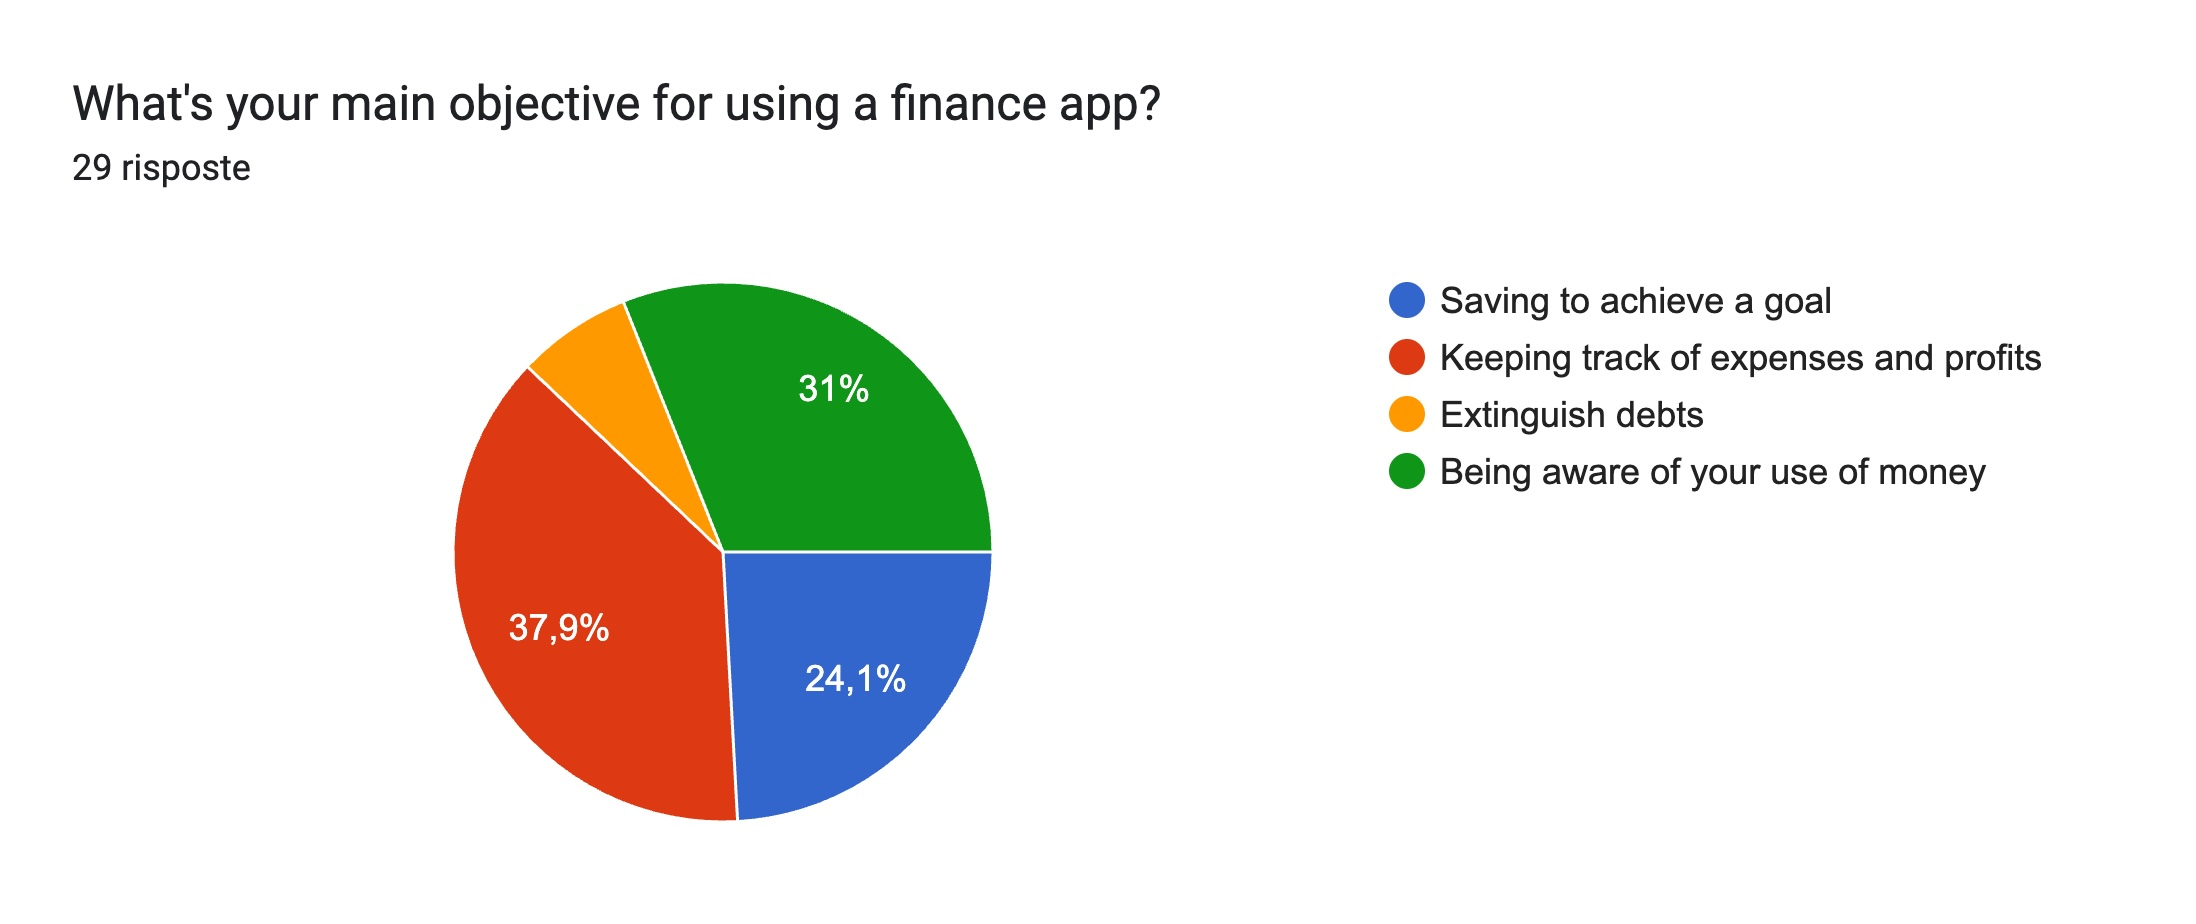
\includegraphics[width=\linewidth]{imagequest1.jpg}
\end{figure}

\begin{figure}[H]
    \centering
    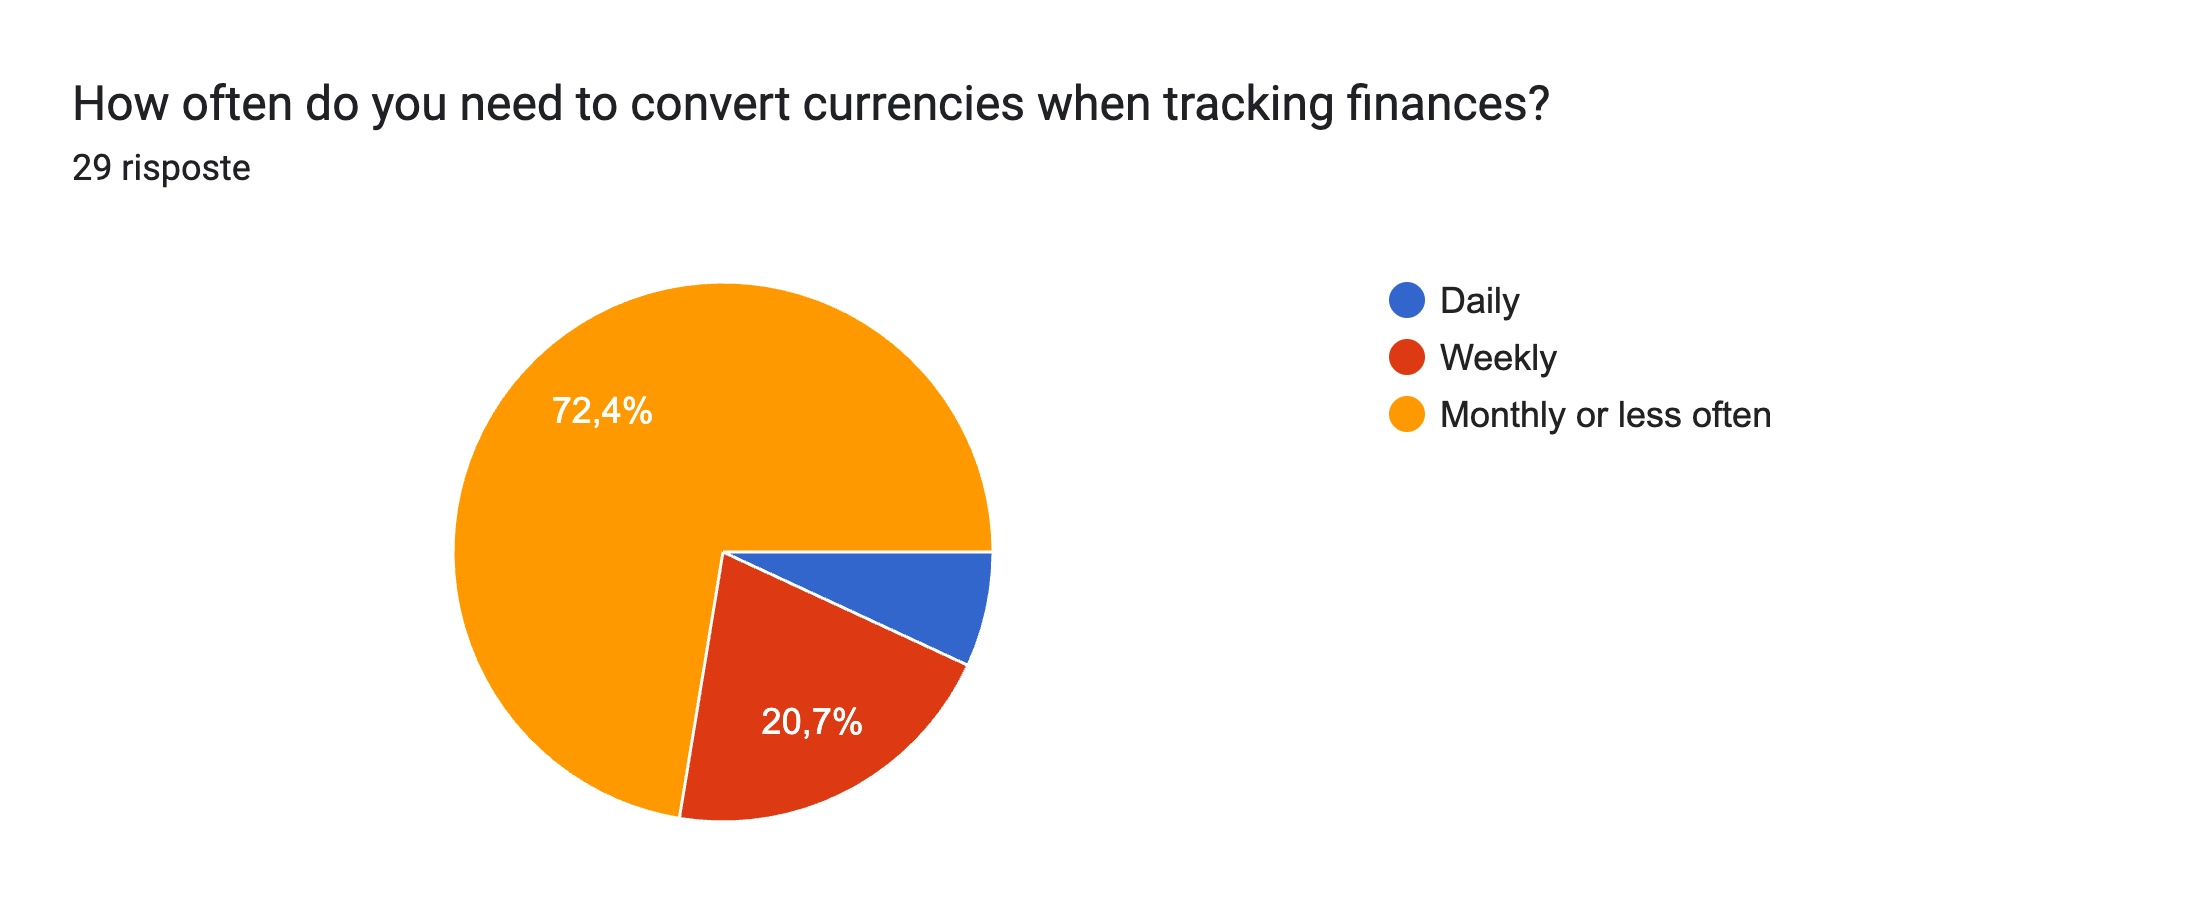
\includegraphics[width=\linewidth]{imagequest2.jpg}
\end{figure}

\begin{figure}[H]
    \centering
    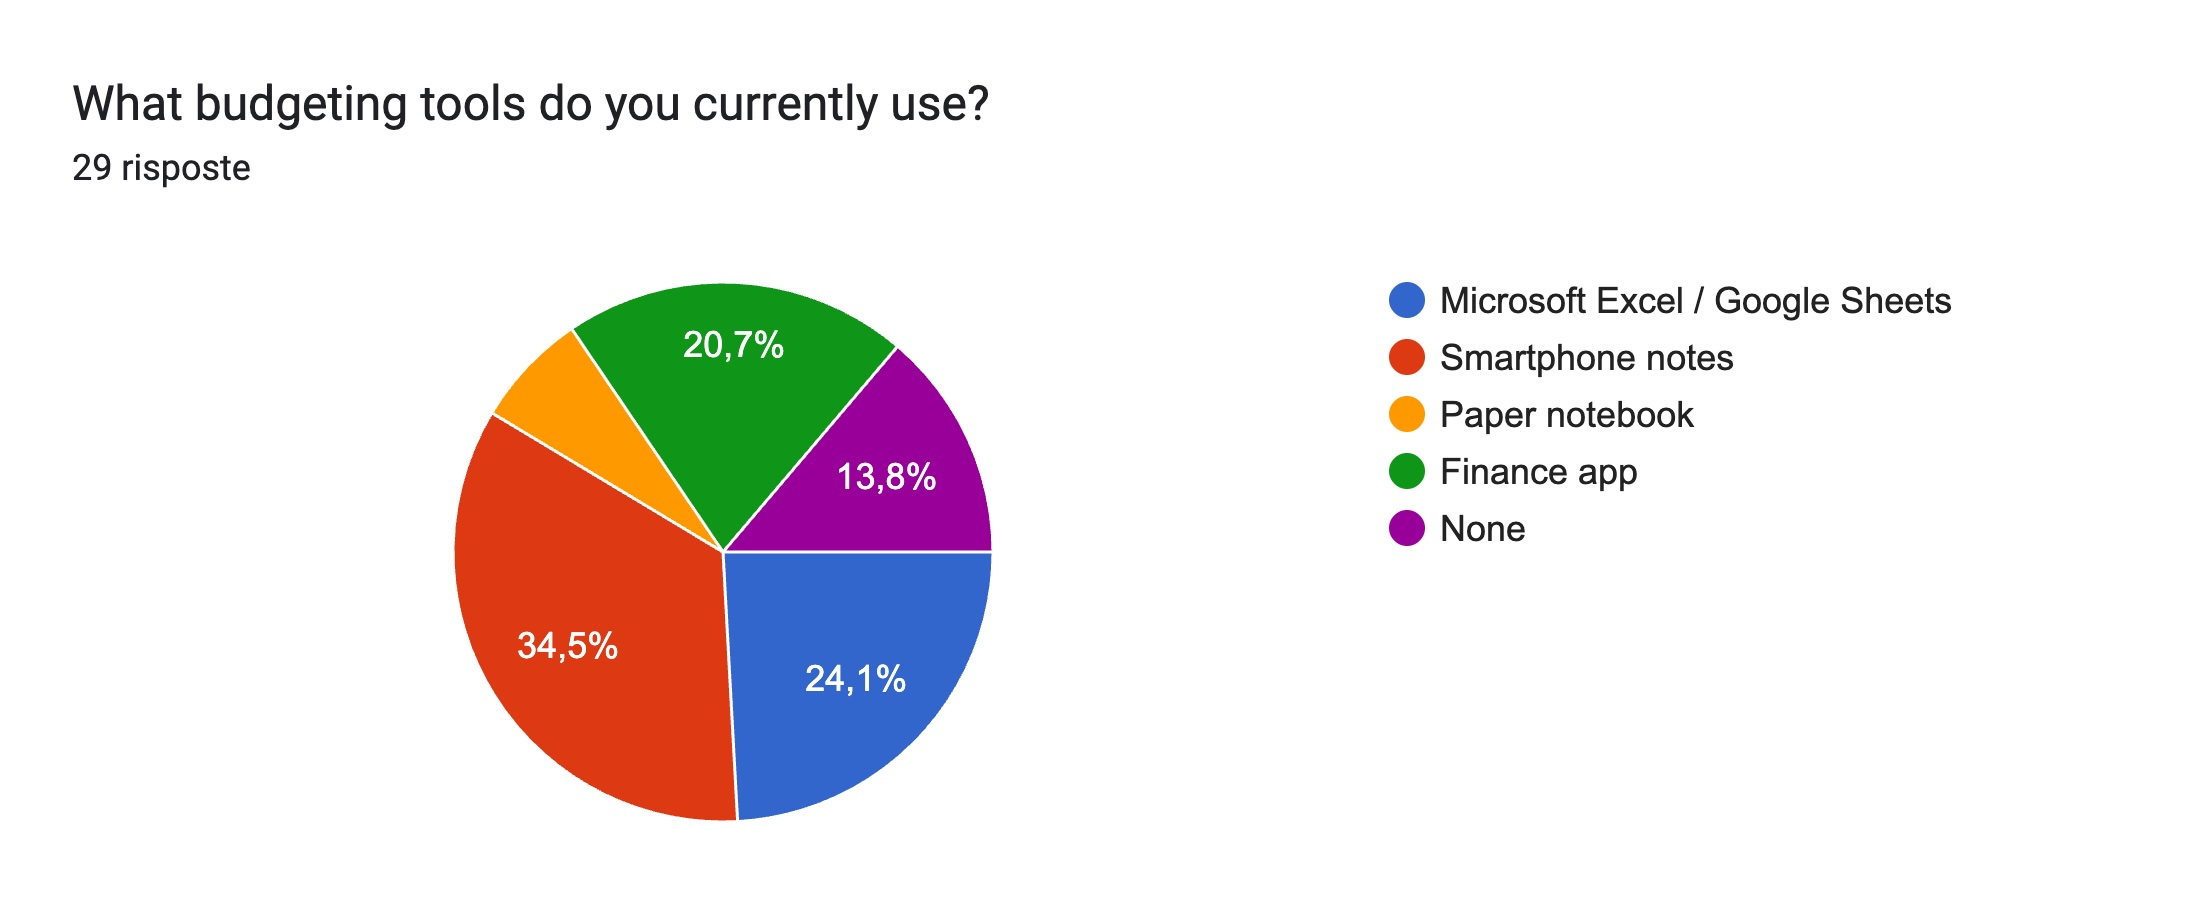
\includegraphics[width=\linewidth]{imagequest3.jpg}
\end{figure}

\begin{figure}[H]
    \centering
    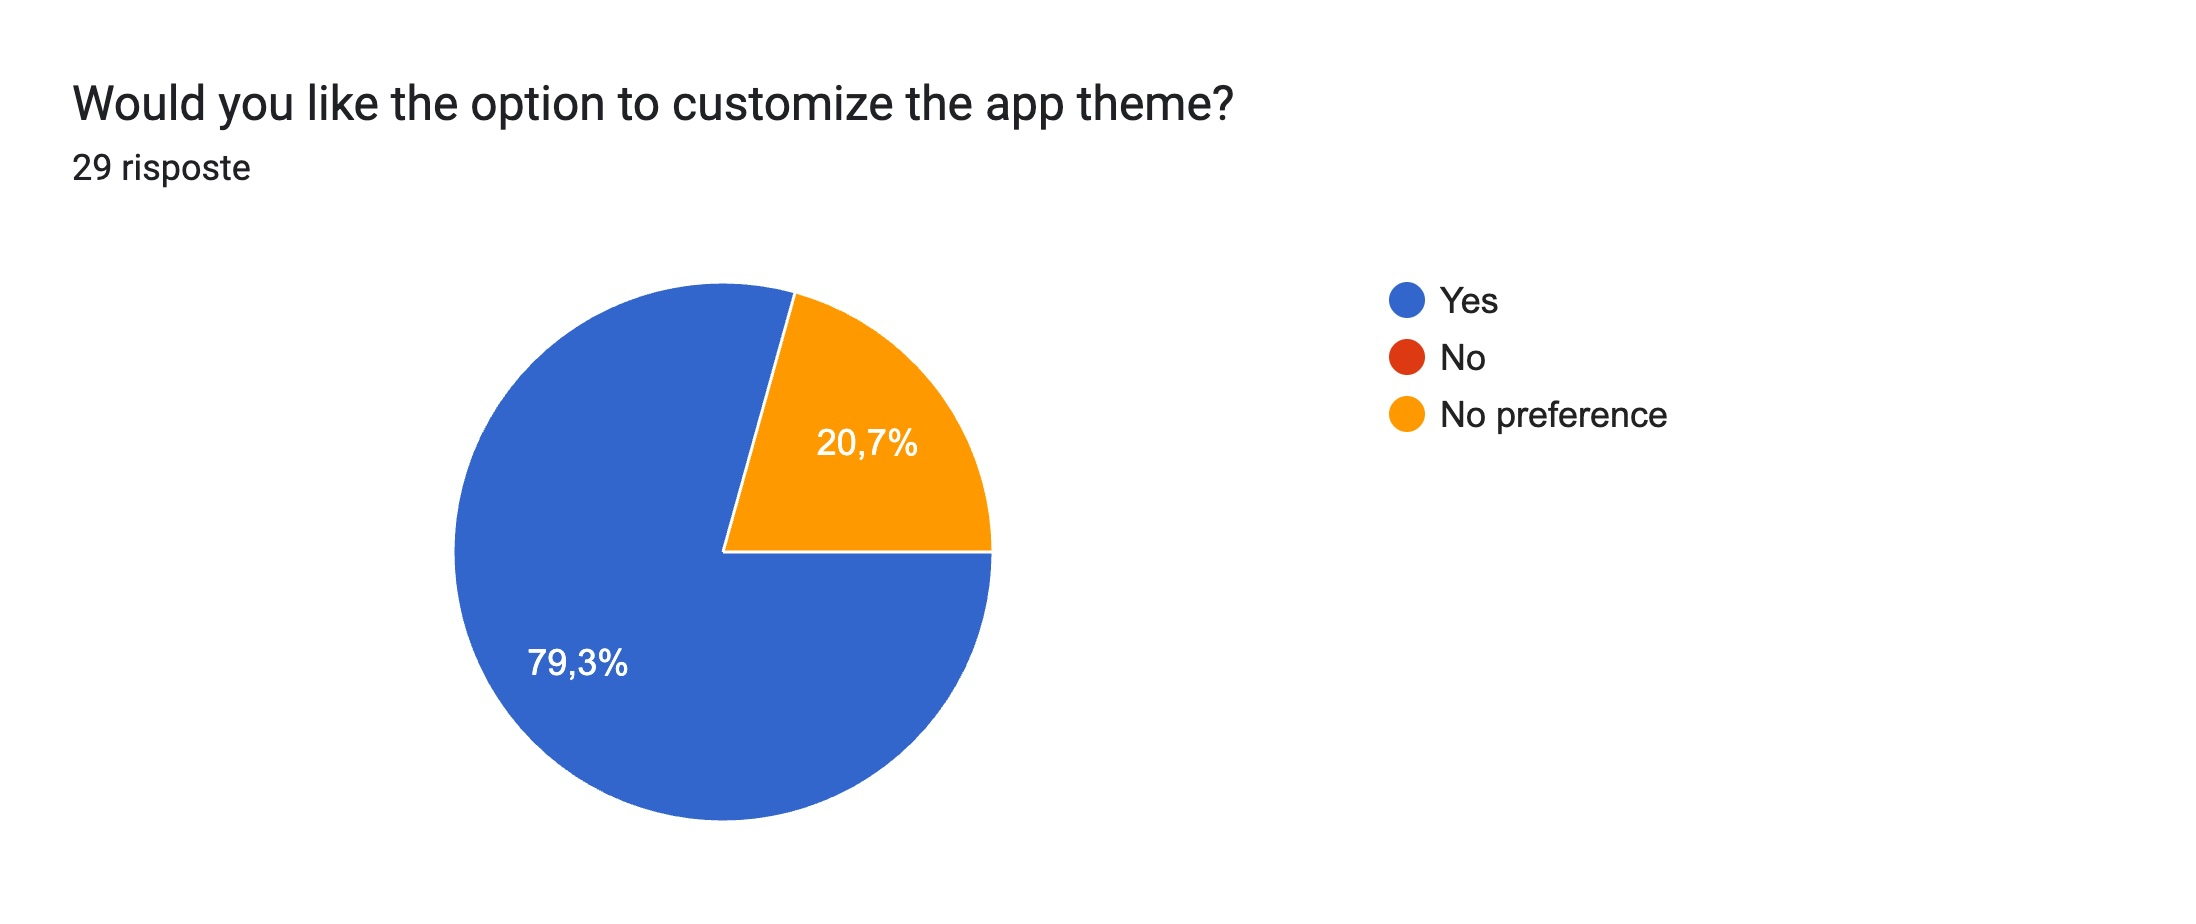
\includegraphics[width=\linewidth]{imagequest4.jpg}
\end{figure}

\begin{figure}[H]
    \centering
    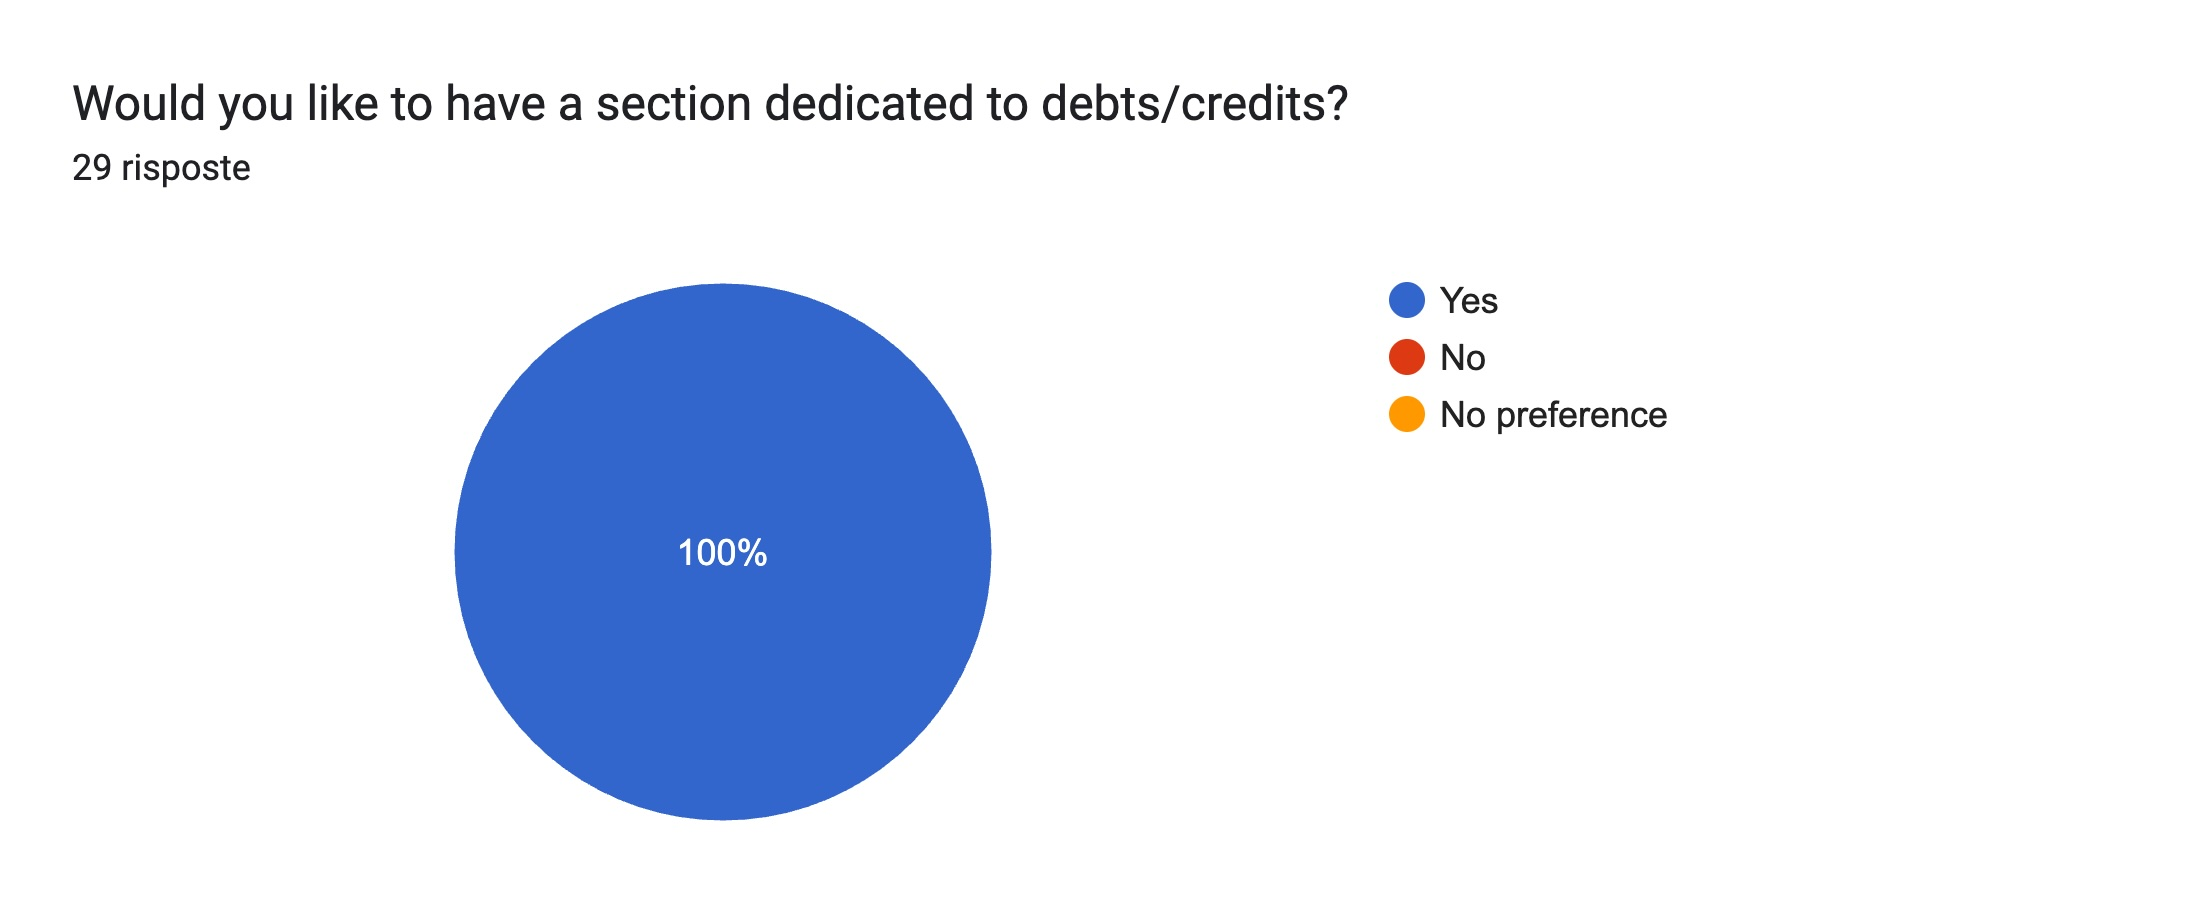
\includegraphics[width=\linewidth]{imagequest5.jpg}
\end{figure}

\begin{figure}[H]
    \centering
    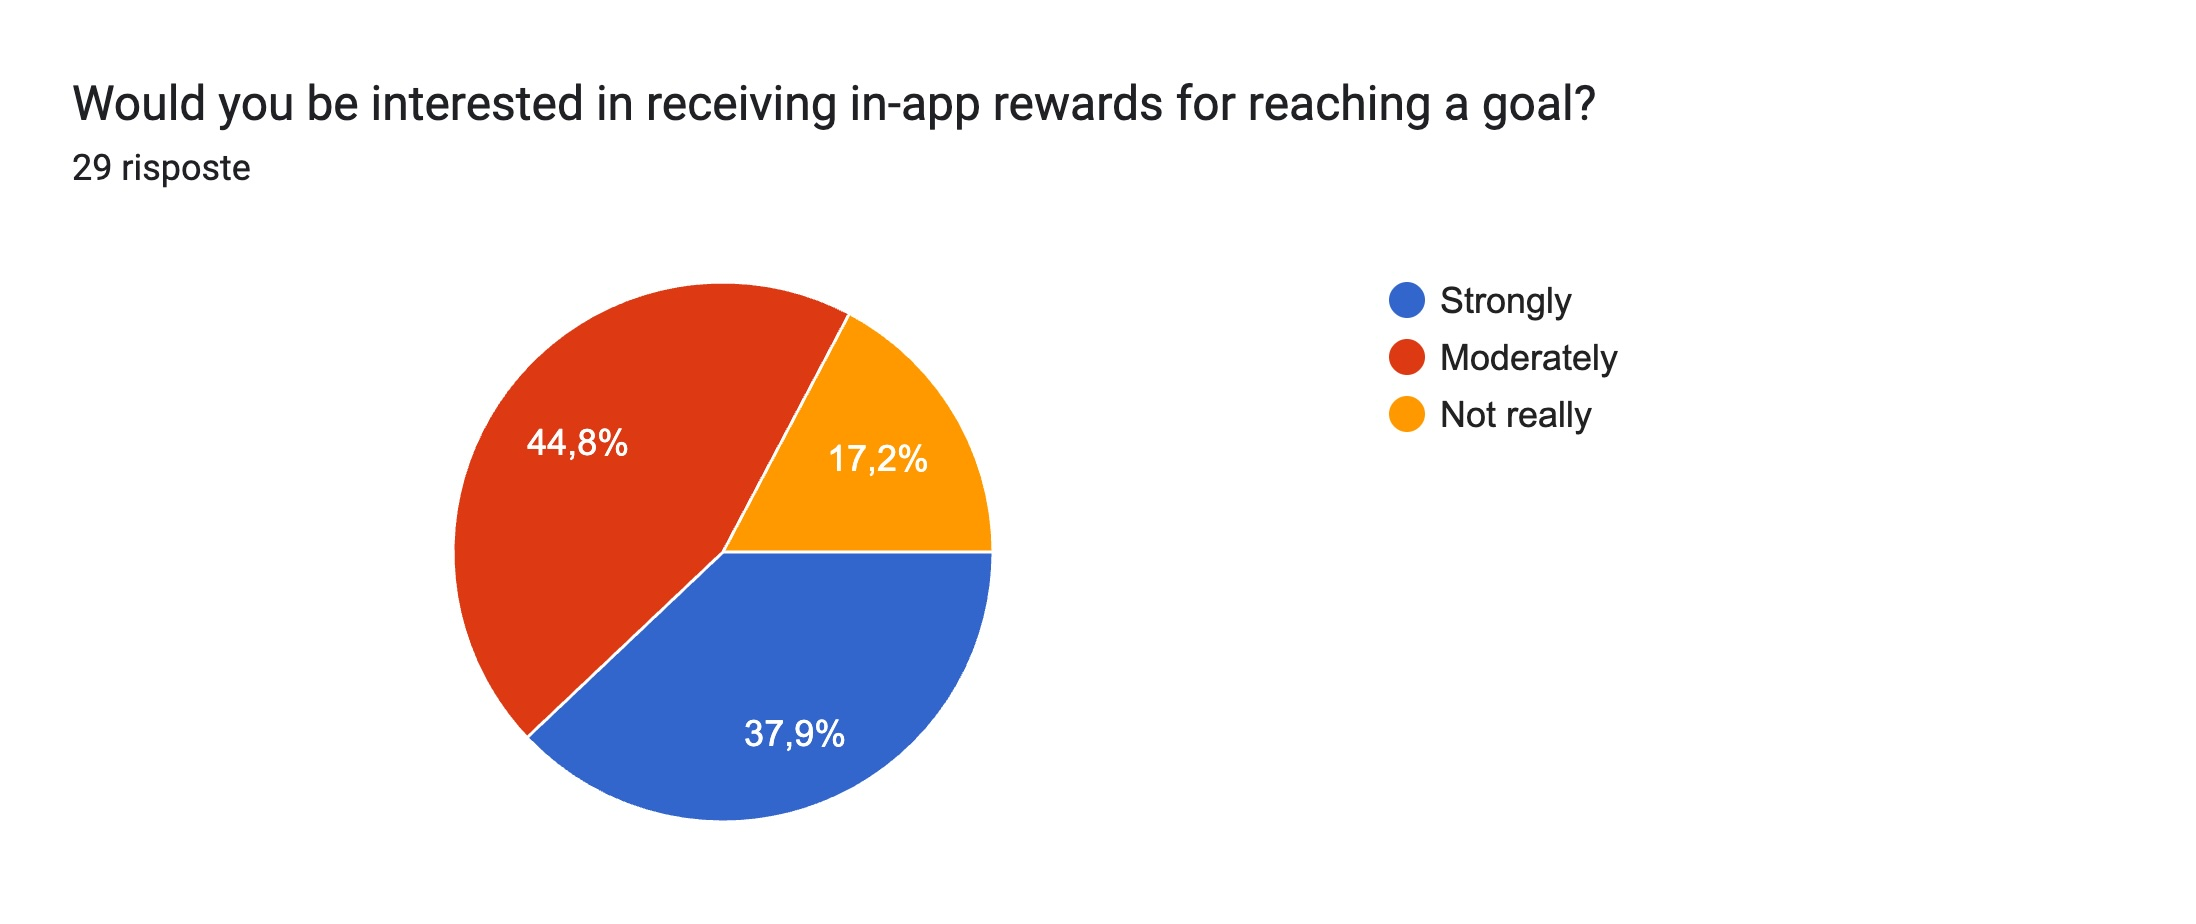
\includegraphics[width=\linewidth]{imagequest6.jpg}
\end{figure}

\begin{figure}[H]
    \centering
    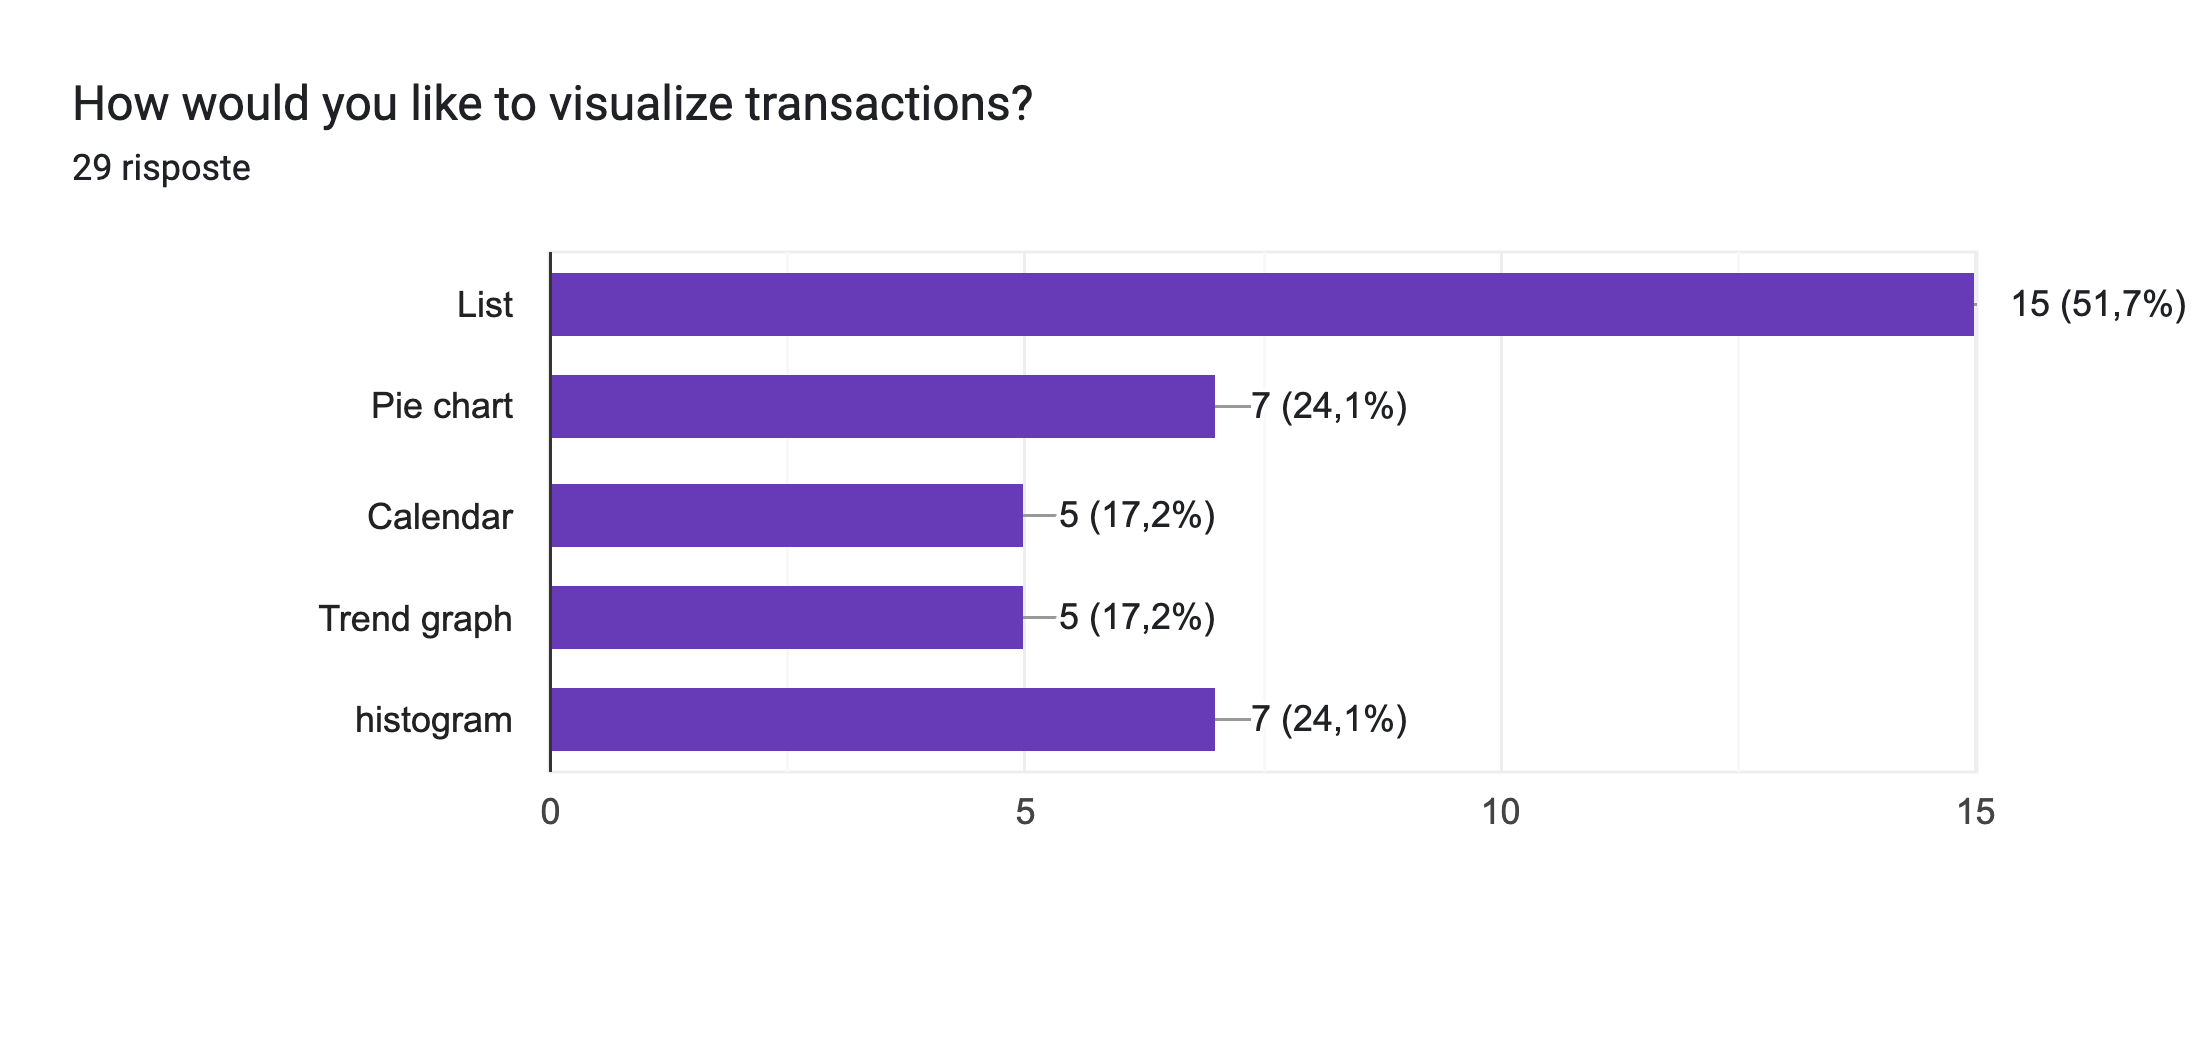
\includegraphics[width=\linewidth]{imagequest7.jpg}
\end{figure}

\begin{figure}[H]
    \centering
    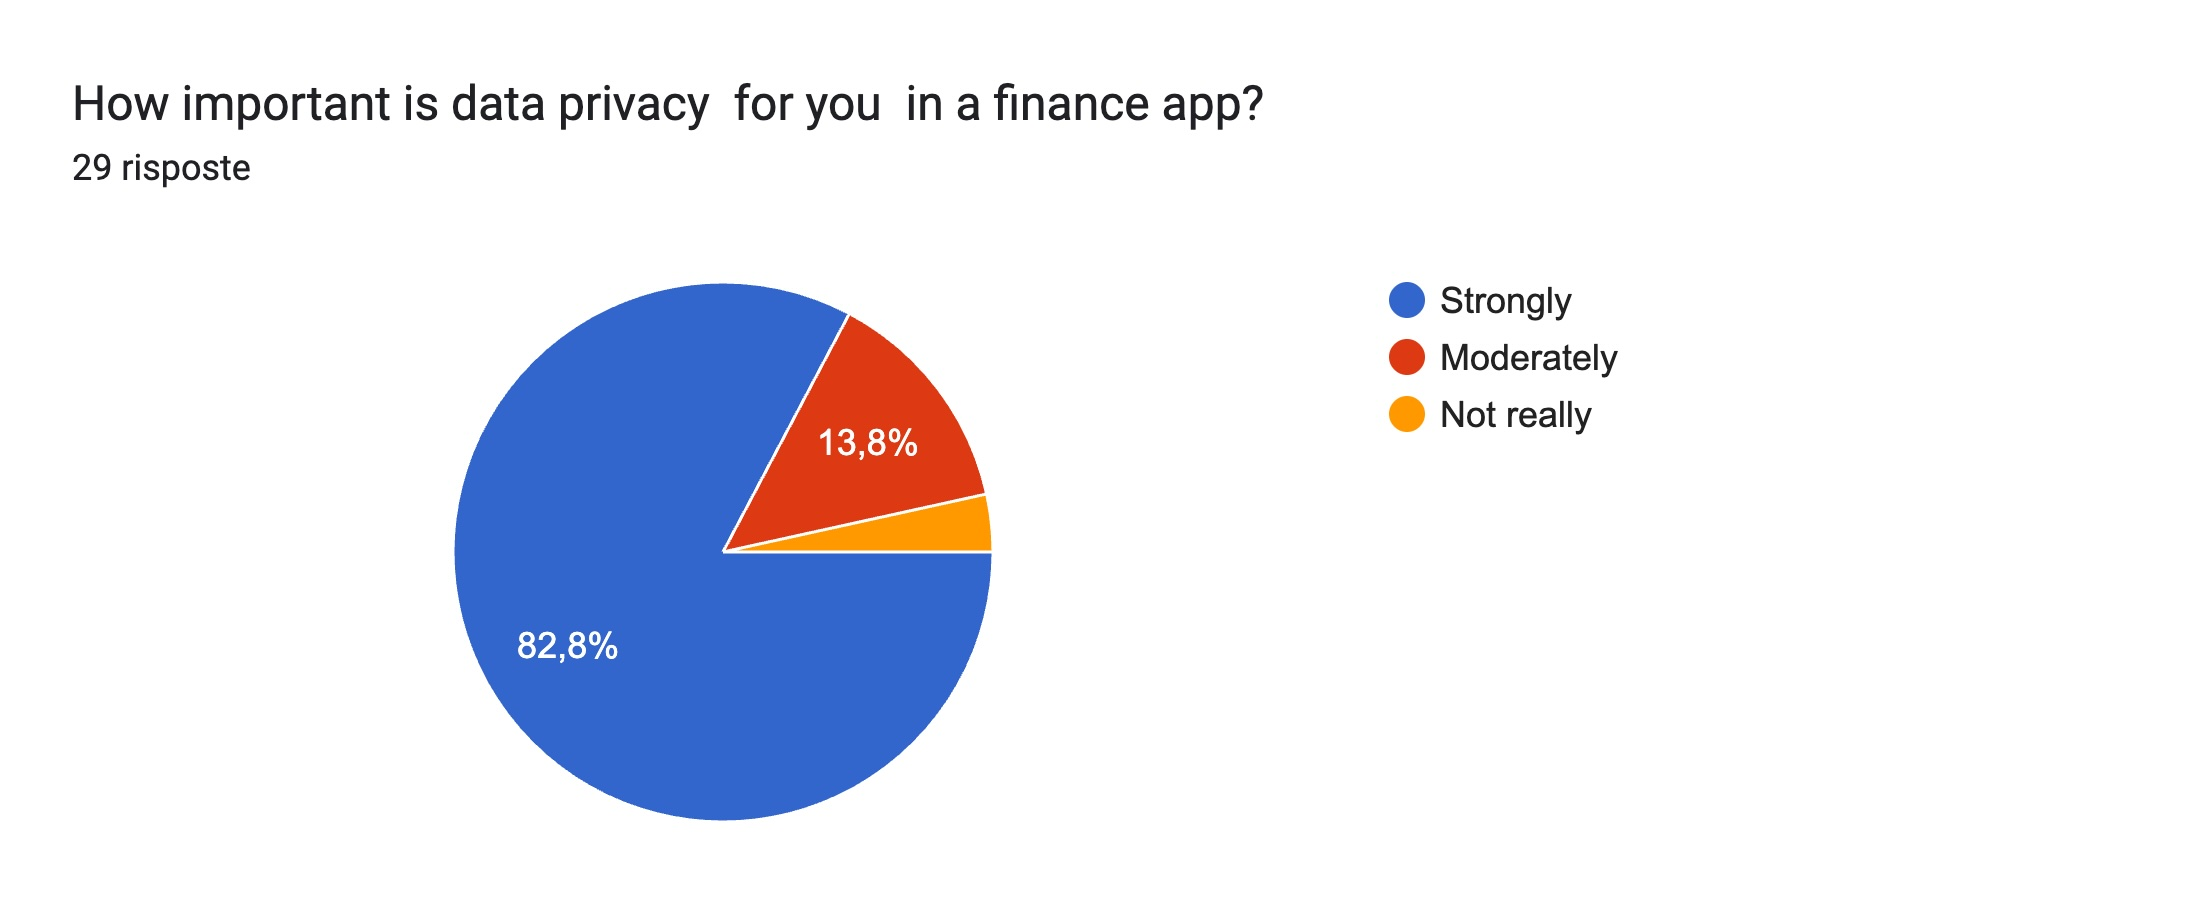
\includegraphics[width=\linewidth]{imagequest8.jpg}
\end{figure}
\noindent In the end we asked "What would stop you from using a finance app?" and we found out that users are primarily deterred from using finance apps by concerns around \textbf{security and privacy}, fearing their financial data might be unsafe or subjected to continuous authentication requests.
\vspace{0.5cm}\\
Beyond security, \textbf{usability is a major hurdle}. Many find apps unnecessarily complicated, not intuitive, or just too difficult to navigate, particularly if the interface feels unhandy. The lack of customization, especially for spending categories, is also a frequent complaint, alongside the annoyance of excessive advertisements.
\vspace{0.5cm}\\
Finally, \textbf{functional limitations} can be a deal-breaker. If an app doesn't support core needs like budgeting, expense tracking, or seamless bank account syncing, or if it requires manual expense entry due to too few spending categories, users will look elsewhere. Some personal barriers, like not feeling capable of using such an app or the app being irrelevant due to a complete lack of funds, also emerged as reasons. Ultimately, if an app doesn't help users achieve their financial goals, they'll simply seek a better alternative.
\subsubsection{Interview}

The feedback from the interviews with users can be synthesized into: Simplicity, Comprehensive Features, and Engaging Motivation.
\begin{itemize}
\item Simplicity and Ease of Use are Paramount
The most consistent piece of feedback, mentioned by a majority of users, is the demand for simplicity. Many current applications are perceived as "too confusing", "overcomplicated" or having a cluttered interface that resembles a spreadsheet.

\item Users want an app that is intuitive from the start, allowing for quick and easy transaction entries without filling out excessive information.
Simple graphs and charts, like pie charts showing expenses by category, are highly valued for understanding spending at a glance.
\item Many users focused on personal goals. They want to set a target (e.g., "Save €500 for a new phone"), track their progress visually, and receive encouraging notifications. The "Duolingo-style" path, where users complete small, consistent steps to reach a larger goal, was cited as a highly appealing model.
\end{itemize}

\subsection{Competitor Analysis}
To better understand our competitors we analyzed the answers from the questionnaire and looked at some of the most downloaded finance apps. These where the apps we analyzed:
\begin{itemize}
    \item Budget e Finanze
    \item Splitwise
    \item Money Manager
    \item 1Money
\end{itemize}
We tried this apps in order to understand their features, strengths and weaknesses.
\begin{figure}[H]
    \centering
    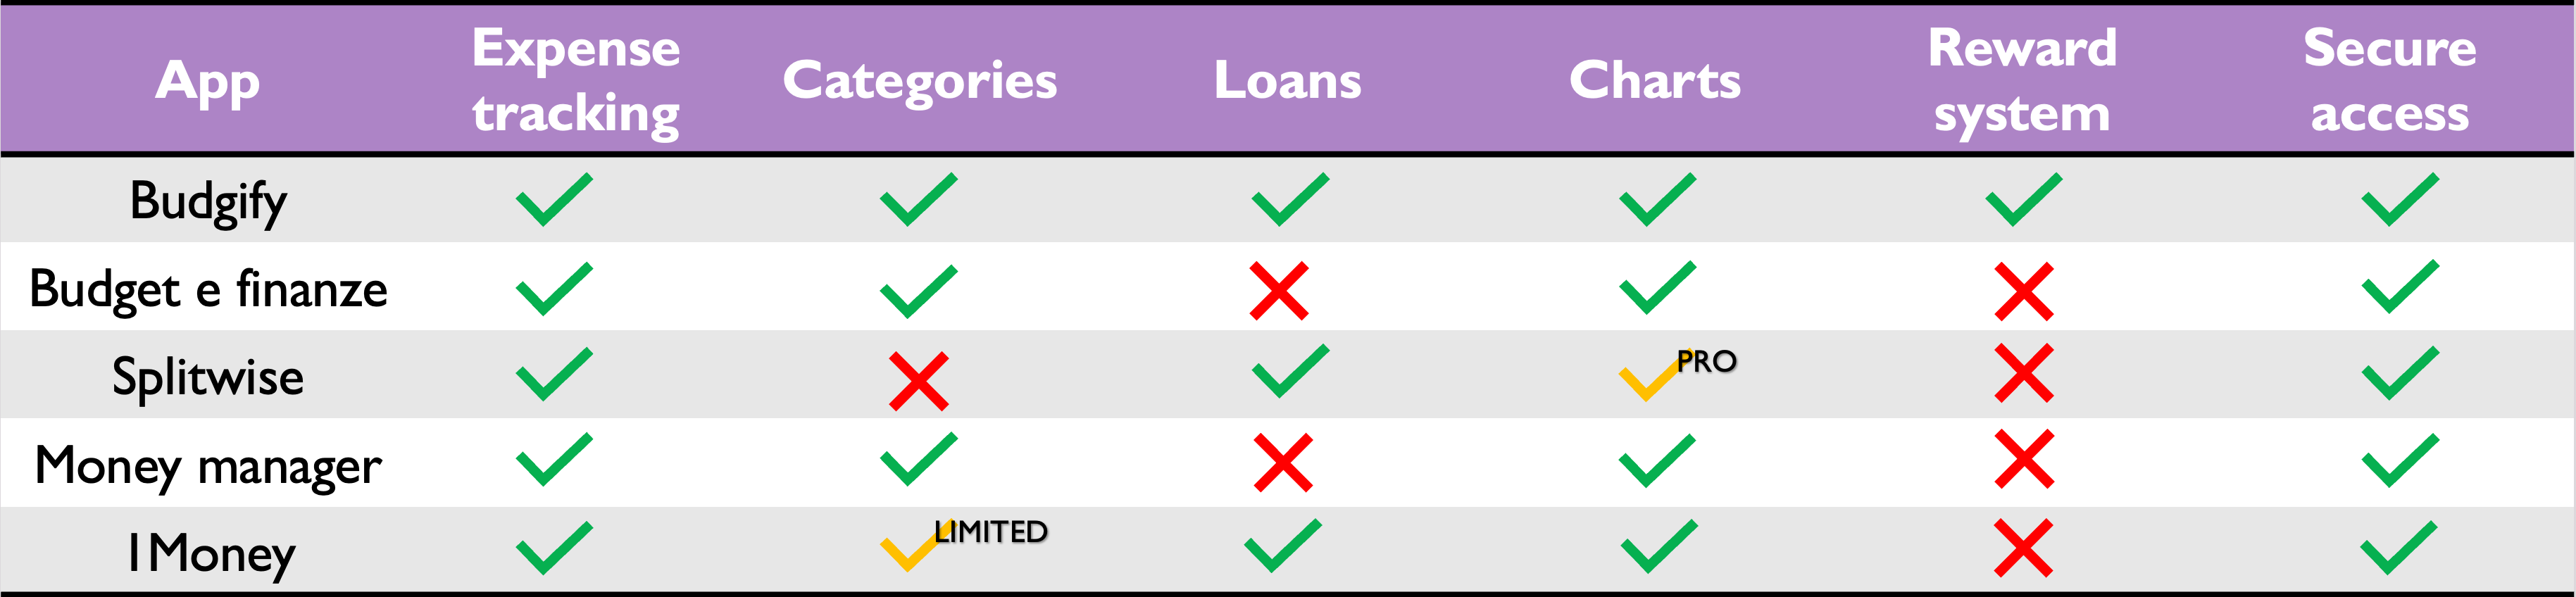
\includegraphics[width=\linewidth]{Competitors_table.png}
\end{figure}
\noindent As we can see all of them offer a basic expense tracking system and a secure access to the app. It's interesting to note that most of the apps offer only one type of chart.\newline \textbf{Budget e finanze} and \textbf{Money Manager} don't feature loans management.\newline \textbf{Splitwise} is missing category personalization and provides charts only in the PRO version.\newline \textbf{1Money} allows the creation of a limited number of categories without paying for the pro version.\newline All of them lack a rewarding system that is helpful to keep the user interested in using the application.\newline Considering this analysis we decided to focus on giving all the functionalities and adding an engaging reward system.
\subsection{Hierarchical Task Analysis}

Hierarchical Task Analysis (HTA) is a task description methodology that is used to produce a complete description of tasks in a hierarchical structure of goals, sub-goals, operations and plans in order
to have a complete representation of the action.

\subsubsection{Buy an item and record the expense}
\begin{figure}[H]
    \centering
    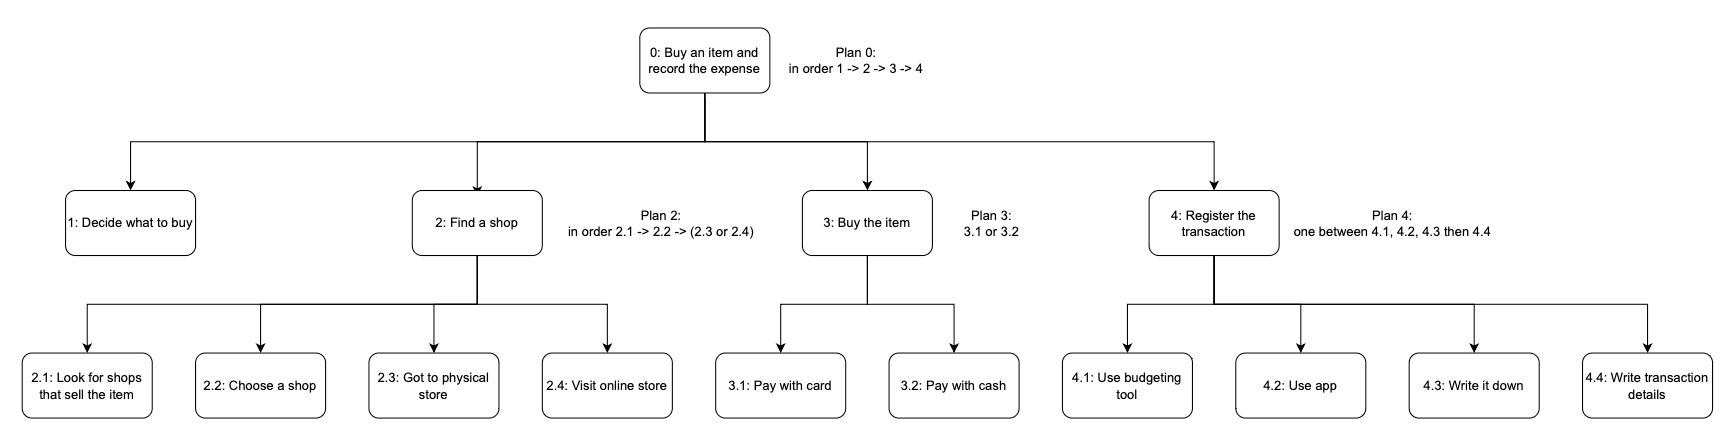
\includegraphics[width=\textwidth]{HTA1.png}
\end{figure}

\subsubsection{Set an objective and buy the related item}
\begin{figure}[H]
    \centering
    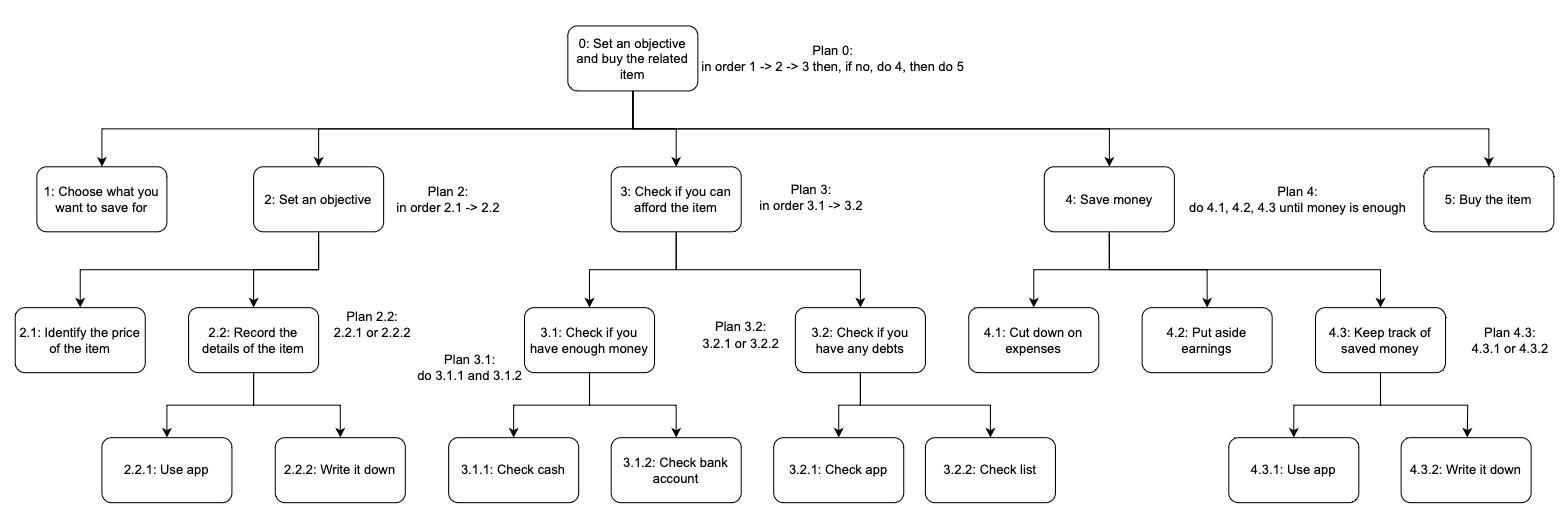
\includegraphics[width=\linewidth]{HTA2.png}
\end{figure}

\subsubsection{Extinguish a debt}
\begin{figure}[H]
    \centering
    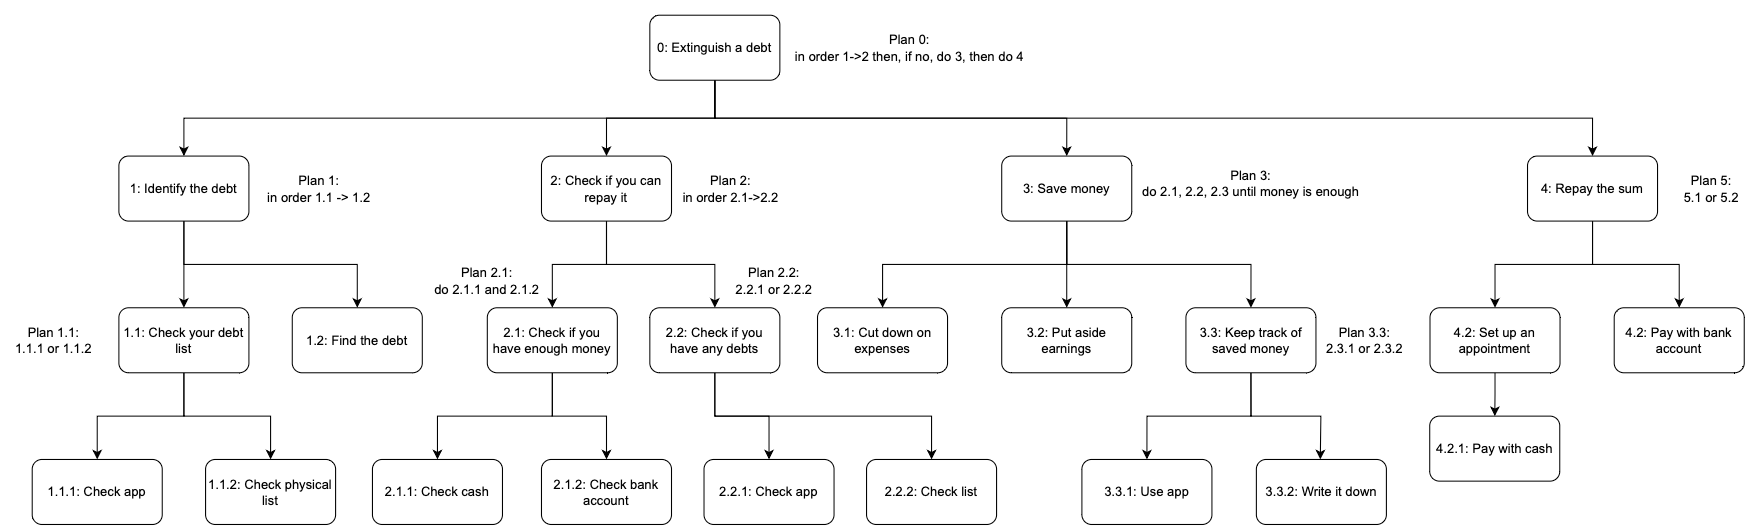
\includegraphics[width=\linewidth]{HTA3.png}
\end{figure}



\subsection{Conclusions Analysis}

In conclusion, the analysis indicates a clear user need for a comprehensive and goal-oriented financial tool. The application's core functionality should be built around motivating users through rewarding reaching Goals, transforming saving from a chore into an engaging challenge. To provide a complete financial picture, robust Debts and Credits handling is essential. Proactive financial planning will be enabled by a Transactions Calendar, which helps users anticipate future payments and deadlines. For insightful analysis of spending habits, the app must provide clear Percentages on kinds of purchases. Underpinning all of this is the fundamental need for user control, allowing individuals to seamlessly Create, Delete, or Change accounts, ensuring the tool remains flexible and perfectly tailored to their evolving financial lives.
\vspace{5cm}
\section{Design and Implementation}
State Transition Network (STN) represents a dialogue between the user and the sys-
tem, in which the system could support the tasks that the customer has to execute. It describes
which are the available actions at a certain point, and the consequent state that the system will reach.
\subsection{Add transaction}
The most performed task in the application. The user after an expense or after reciving an income records the transaction on the app.
\begin{figure}[H]
    \centering
    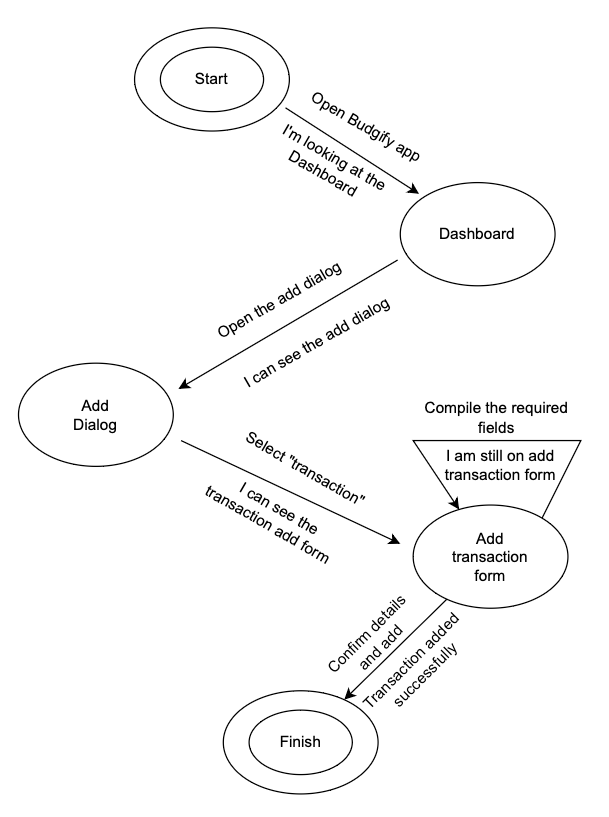
\includegraphics[scale=0.5]{STN1.png}
\end{figure}
\vspace{5cm}
\subsection{Set objective to buy an item}
Here we see how we can set our goal and complete it.
\begin{figure}[H]
    \centering
    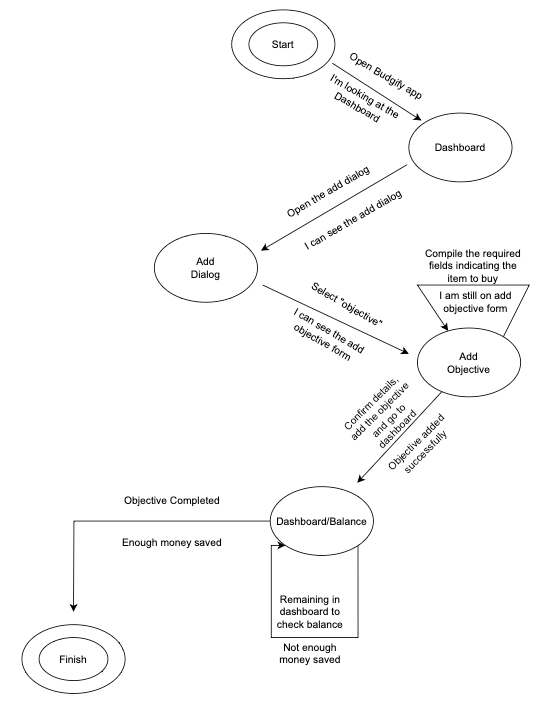
\includegraphics[scale=0.7]{STN2.png}
\end{figure}
\vspace{5cm}
\subsection{Extinguish a debt}
Finally the loan management for a debt, we see how to record the repayment.
\begin{figure}[H]
    \centering
    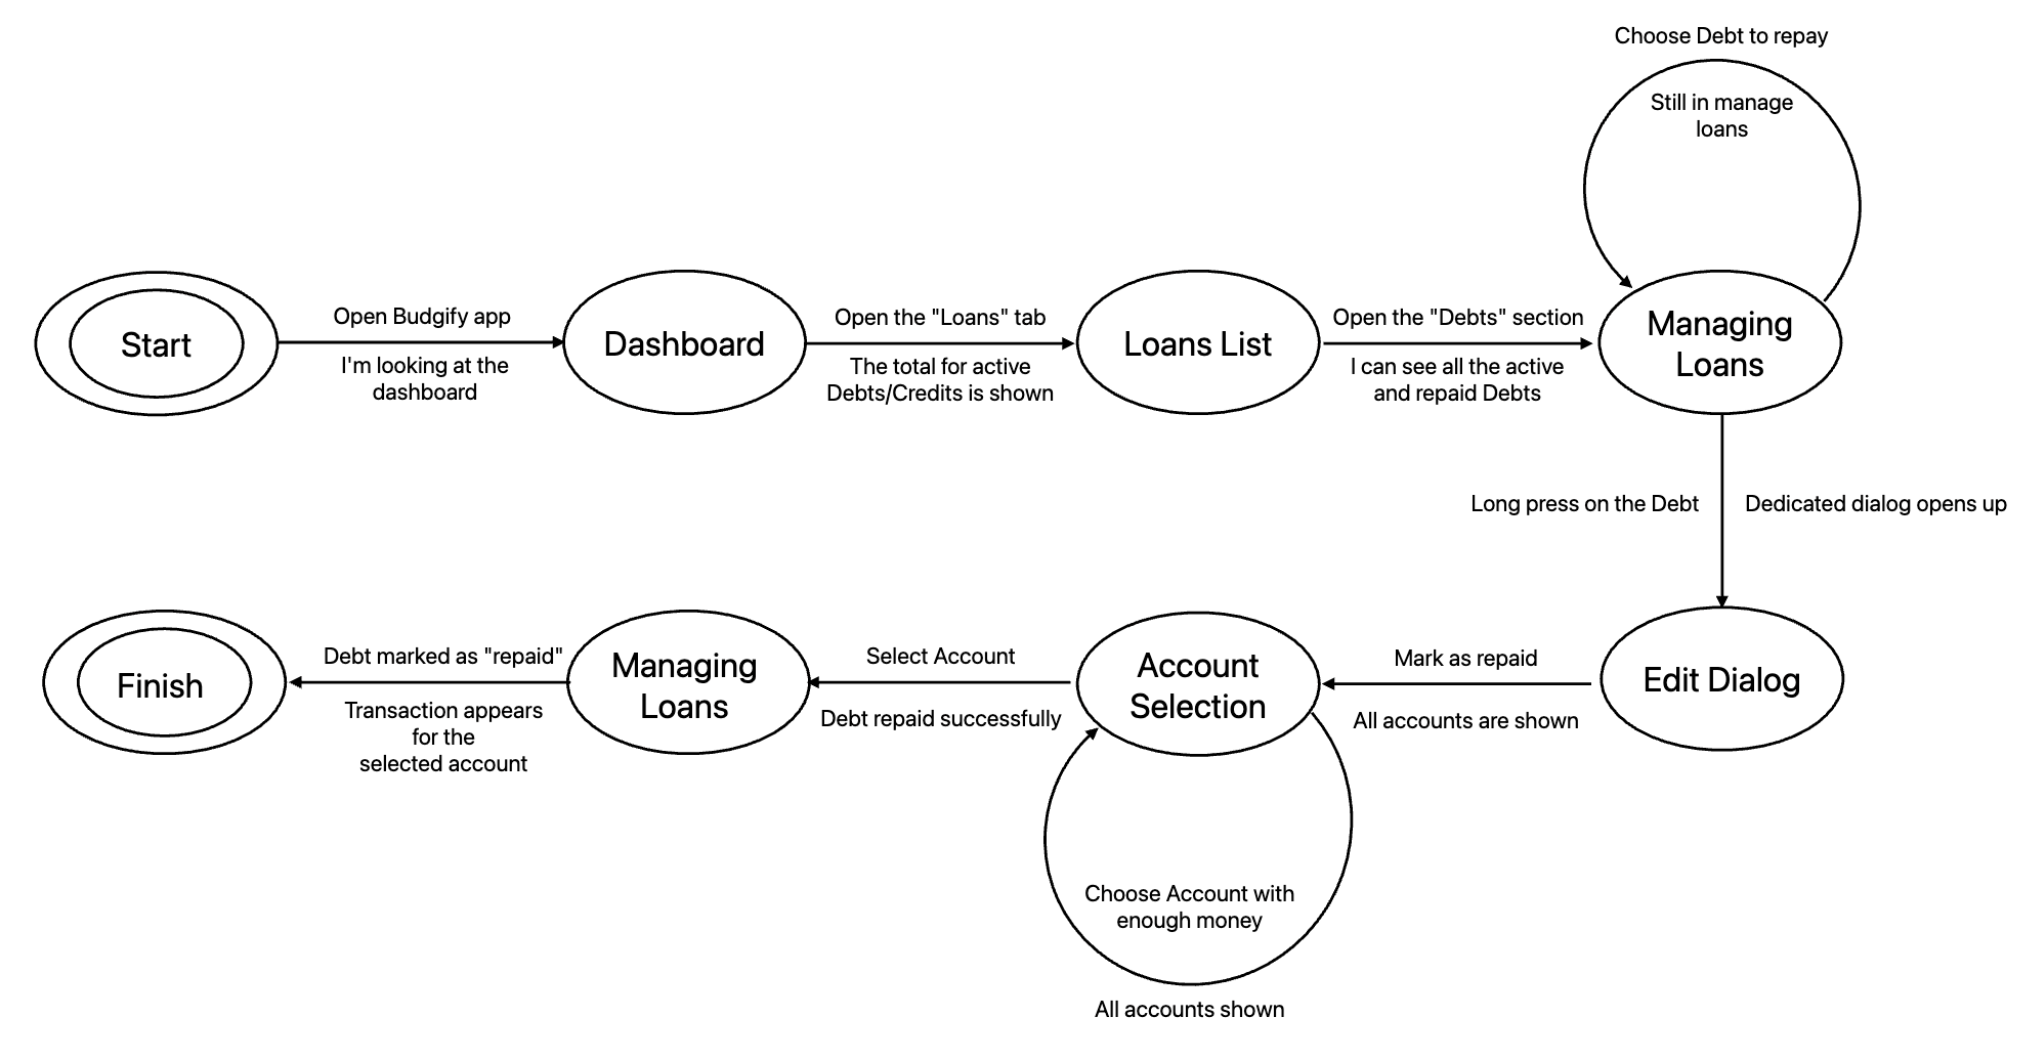
\includegraphics[width=\linewidth]{STN3.png}
\end{figure}

\section{Prototypes}
The next focus is on creating a starting point, an initial mockup to understand how the system reacts to the interaction with the user. Then we transformed this mockups into a fully functional application.
\subsection{Prototype ZERO}
This mockup shows the first iteration of the different screen interfaces:
\begin{itemize}
    \item \textbf{Dashboard:} this is the landing page of the app, a homepage where the user has an overview of what's going on in his finances. It's always reachable trough the "home" icon in the top left corner. From here the user can navigate into the app using the navigation bar at the bottom that leads to the other sections of the application.
    \begin{figure}[H]
        \centering
        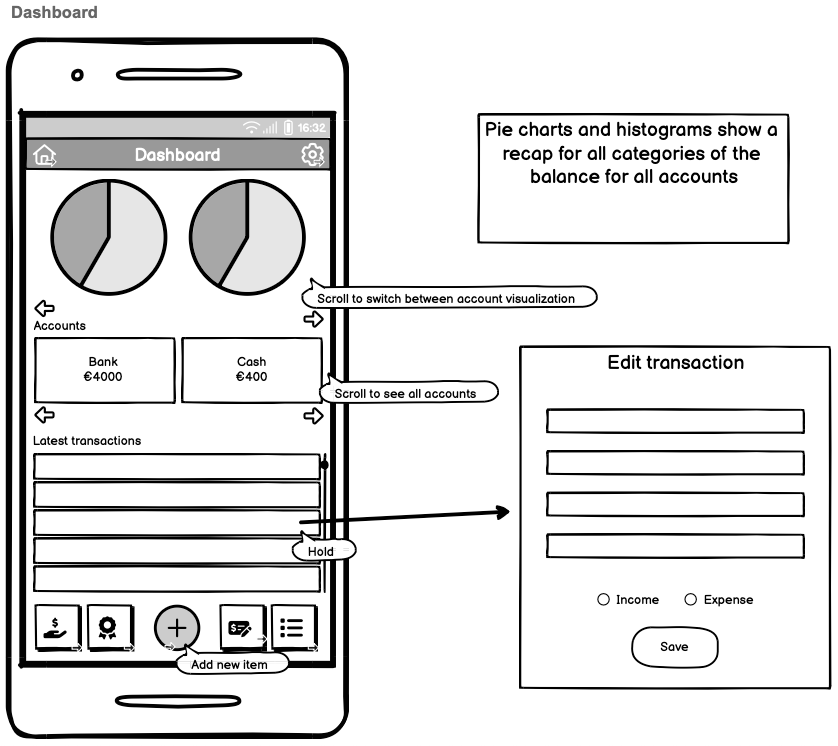
\includegraphics[scale = 0.4]{dashmock.png}
    \end{figure}
    \item \textbf{Transactions:} this is where all the transactions are stored and the user can use the calendar to filter which transactions are displayed.
    \begin{figure}[H]
        \centering
        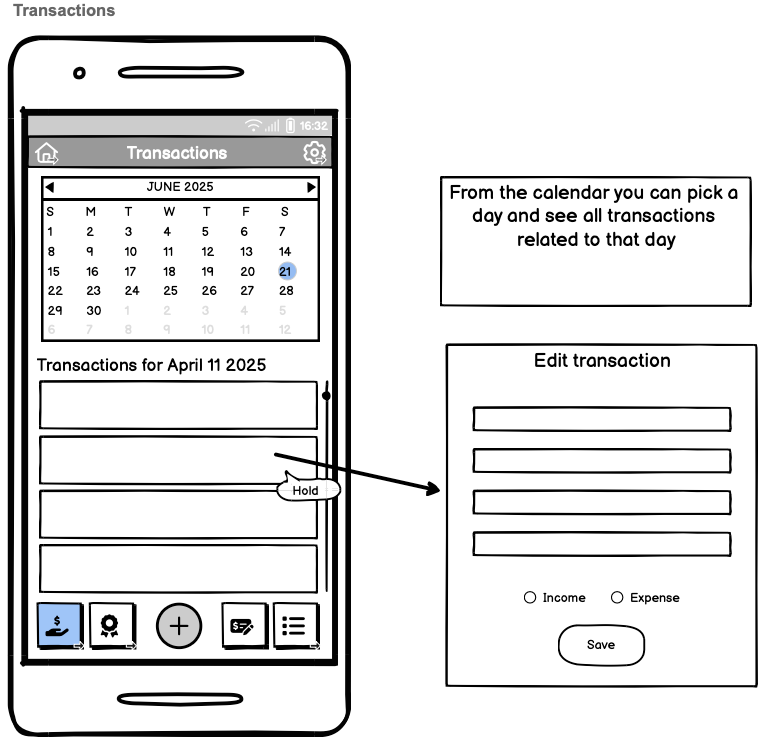
\includegraphics[scale = 0.4]{transmock.png}
    \end{figure}
    \item \textbf{Objectives:} this section is dedicated to the user, to track his progress in saving by setting new goals to reach. By entering the managing page he can see all the goals set and complete or edit them.
    \begin{figure}[H]
        \centering
        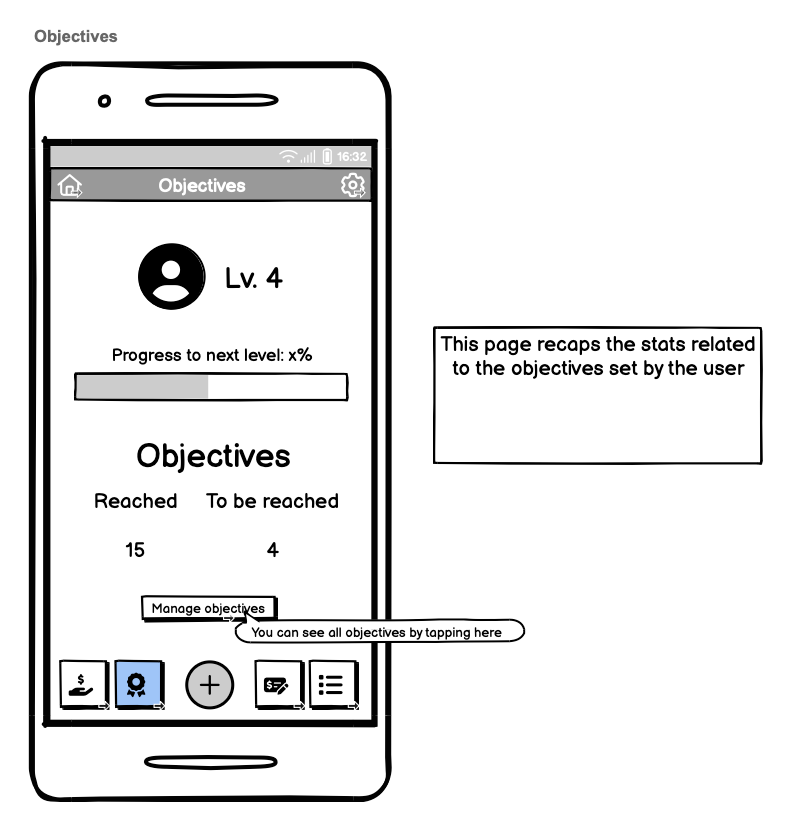
\includegraphics[scale = 0.4]{objmock.png}
    \end{figure}
    \begin{figure}[H]
        \centering
        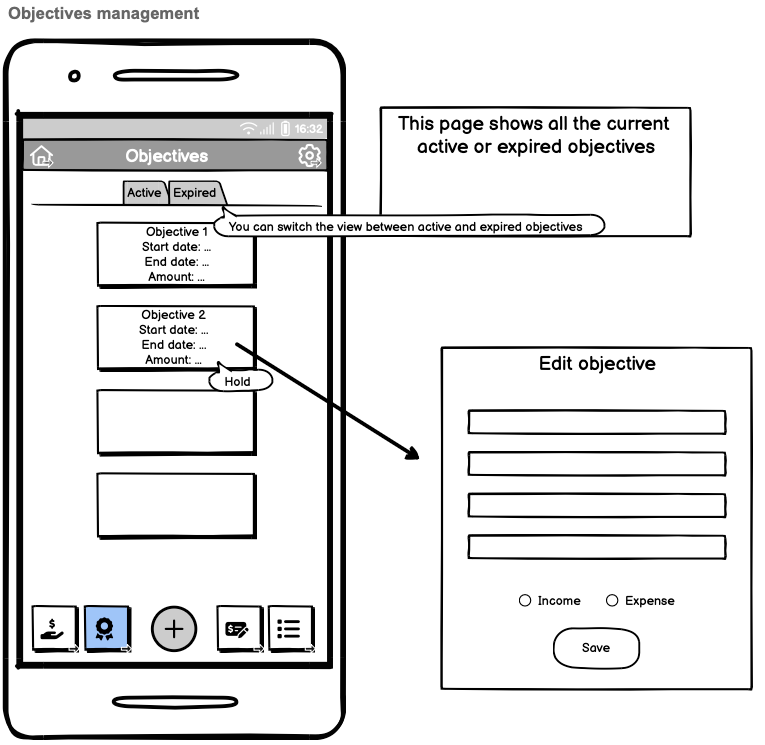
\includegraphics[scale = 0.4]{objmanmock.png}
    \end{figure}
    \item \textbf{Loans:} the user can record lent and borrowed money. And by clicking on the dedicated button on the top can navigate to the management page.
    \begin{figure}[H]
        \centering
        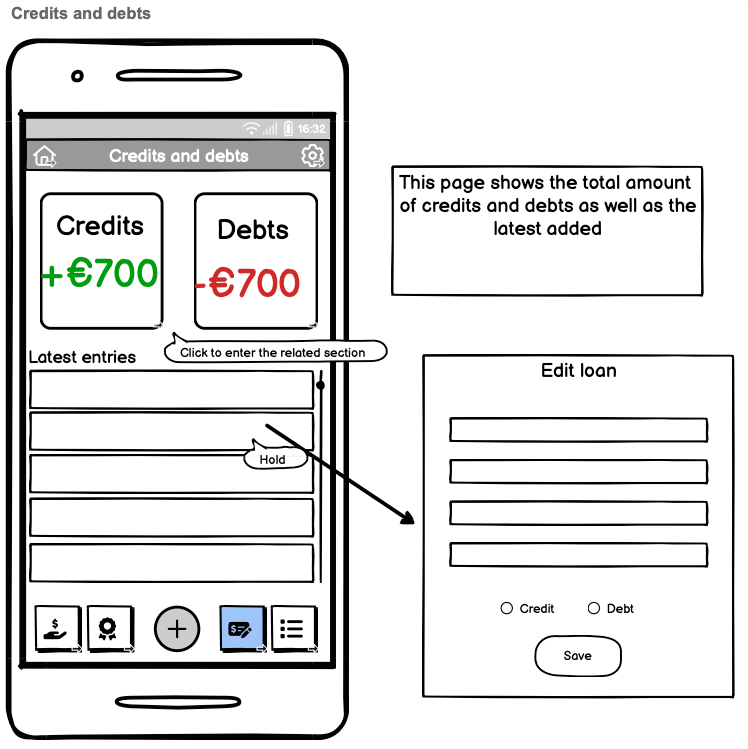
\includegraphics[scale = 0.4]{credebmock.png}
    \end{figure}
    \begin{figure}[H]
        \centering
        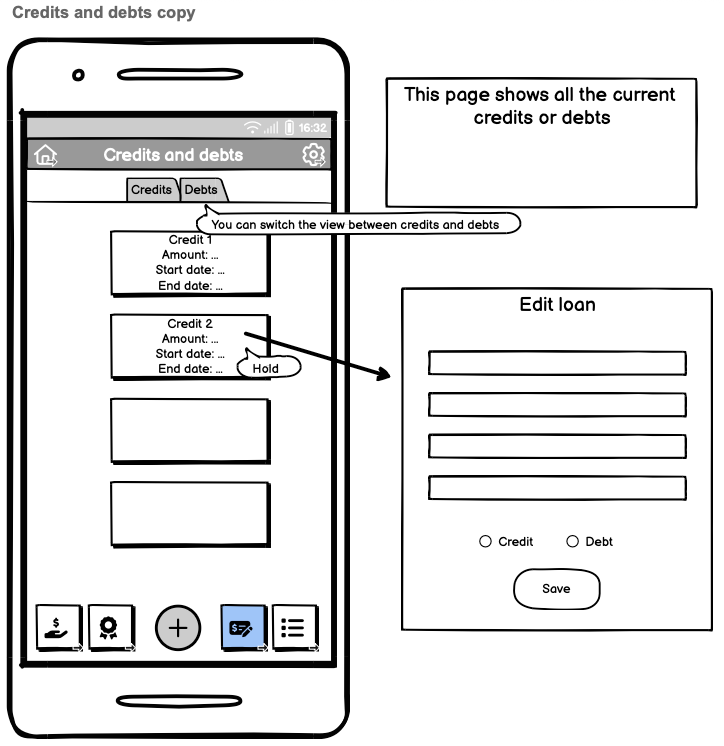
\includegraphics[scale = 0.4]{creddebtmanmock.png}
    \end{figure}
    \vspace{1cm}
    \item \textbf{Categories:} two section for Income and Expenses allow the user to personalize the categorization system.
    \begin{figure}[H]
        \centering
        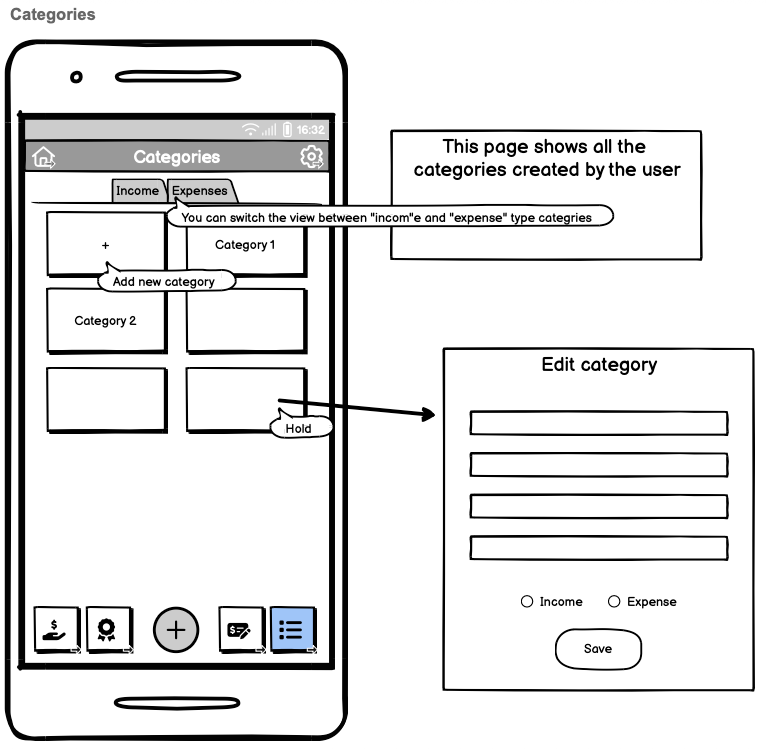
\includegraphics[scale = 0.4]{categmock.png}
    \end{figure}
    \vspace{15cm}
    \item \textbf{Settings:} Finally the settings page to choose the theme of the application, set, delete or change the pin to access the app and other information.
    \begin{figure}[H]
        \centering
        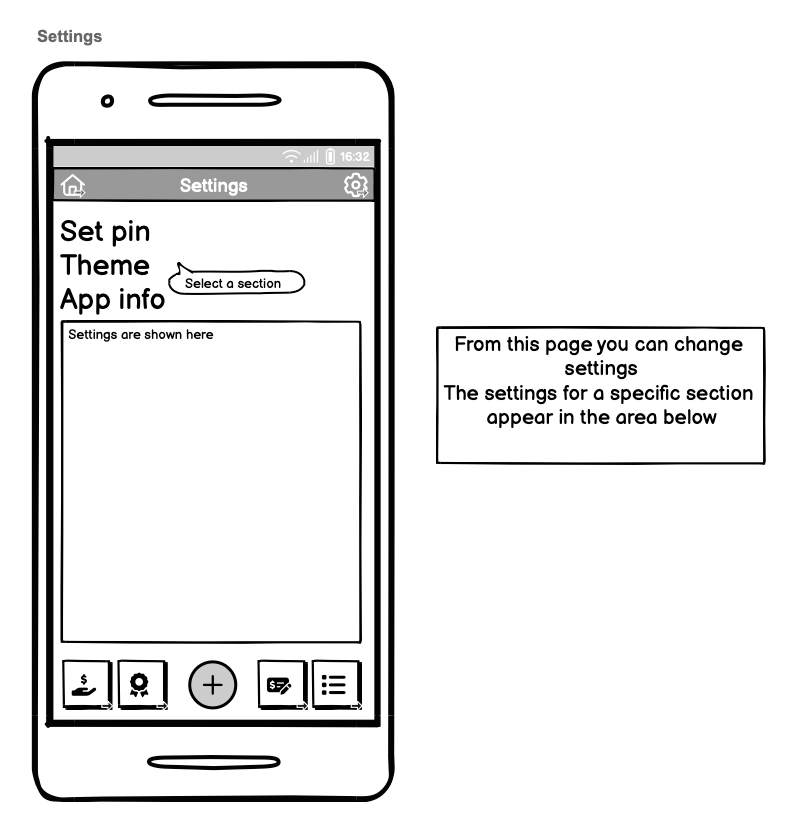
\includegraphics[scale = 0.4]{settmock.png}
    \end{figure}
\end{itemize}
\subsubsection{Expert Evaluation}
Once we finished the first design we requested an Expert Evaluation, to get a professional review of the work done so far. In particular we opted for a Heuristic Evaluation.
\vspace{0.5cm}\\
Usability criteria (heuristics) are identified and design is examined by experts to see if these are
violated. Heuristic Evaluation debugs design highlighting the problems we should solve to achieve better results. The list of criteria is well defined and standardized.\\
We provided our mockup and a brief description of the functionalities and we received an evaluation of the critical aspects.
\begin{figure}[H]
    \centering
    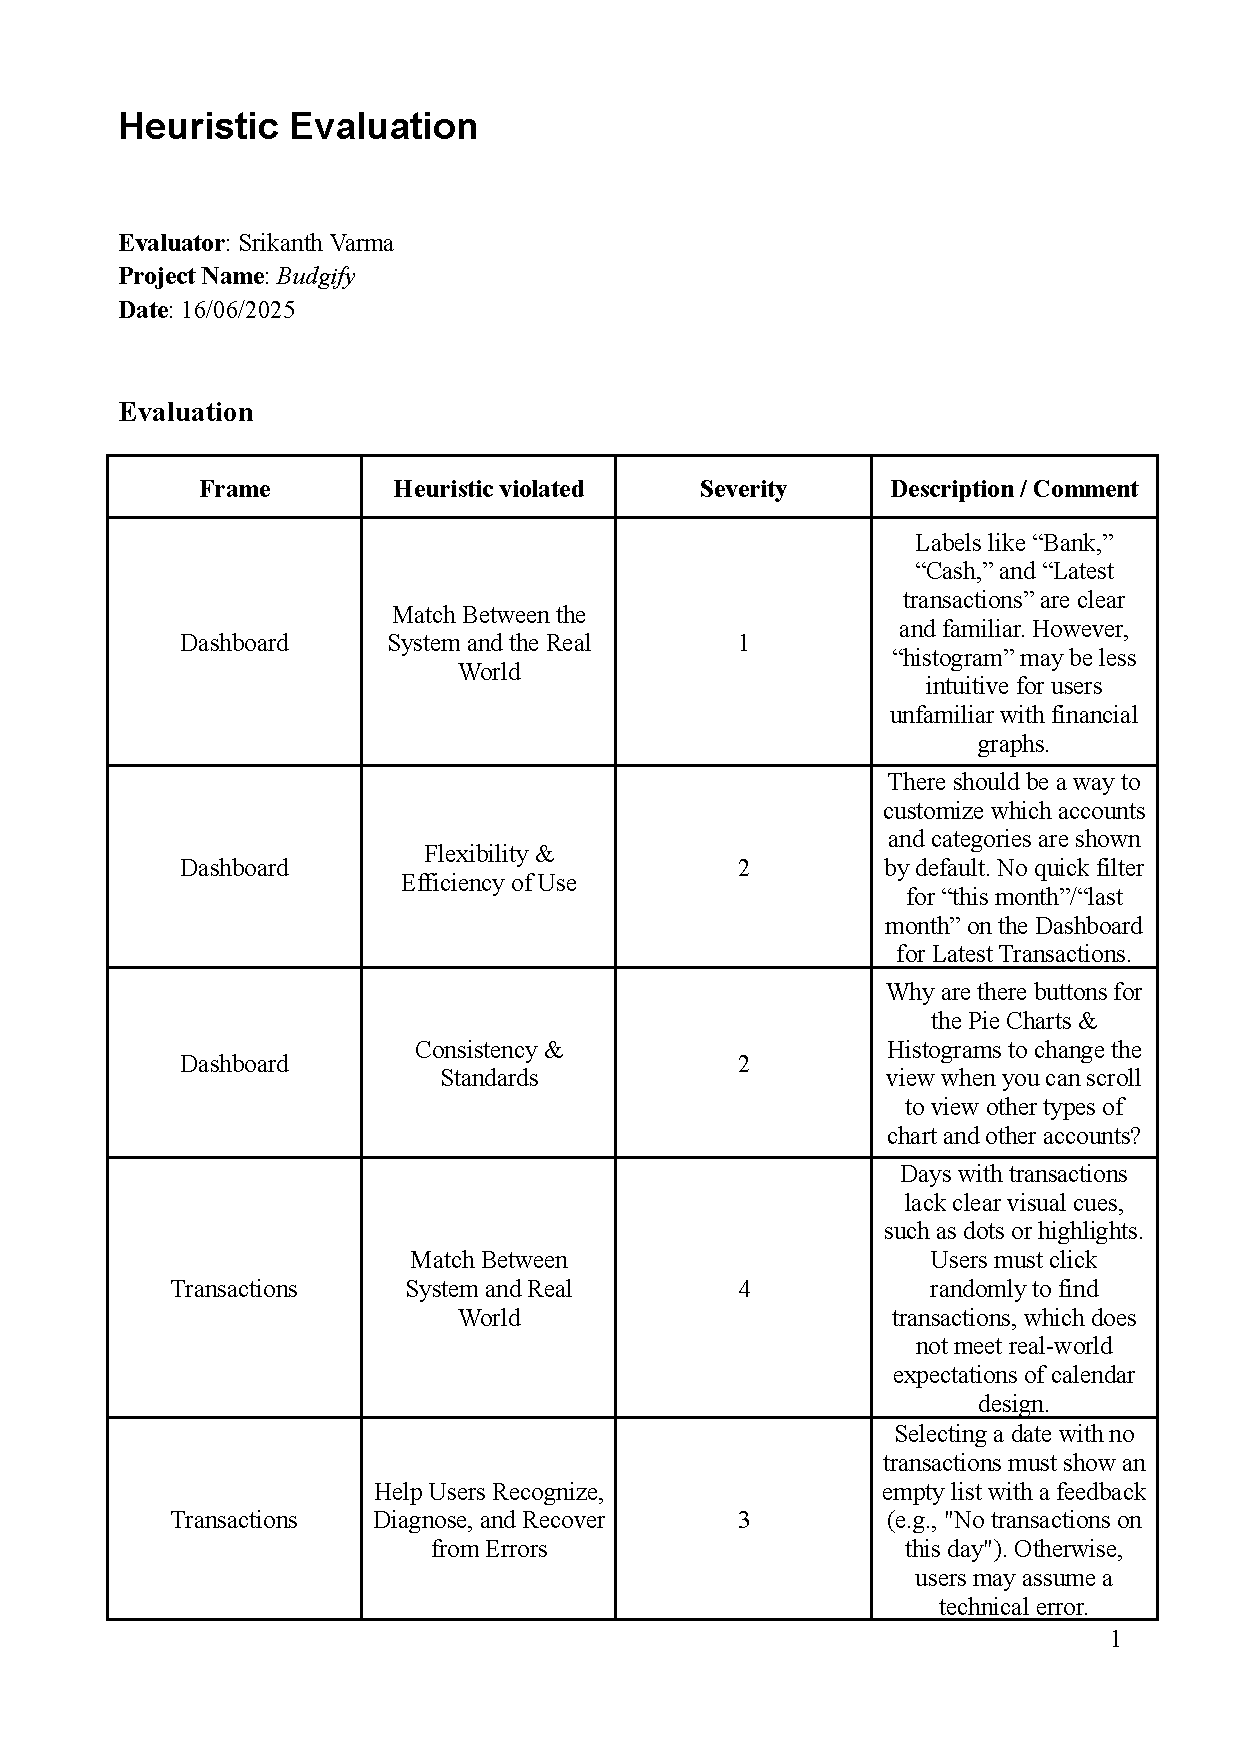
\includegraphics[width=1\linewidth]{HE1.pdf}
\end{figure}
\begin{figure}[H]
    \centering
    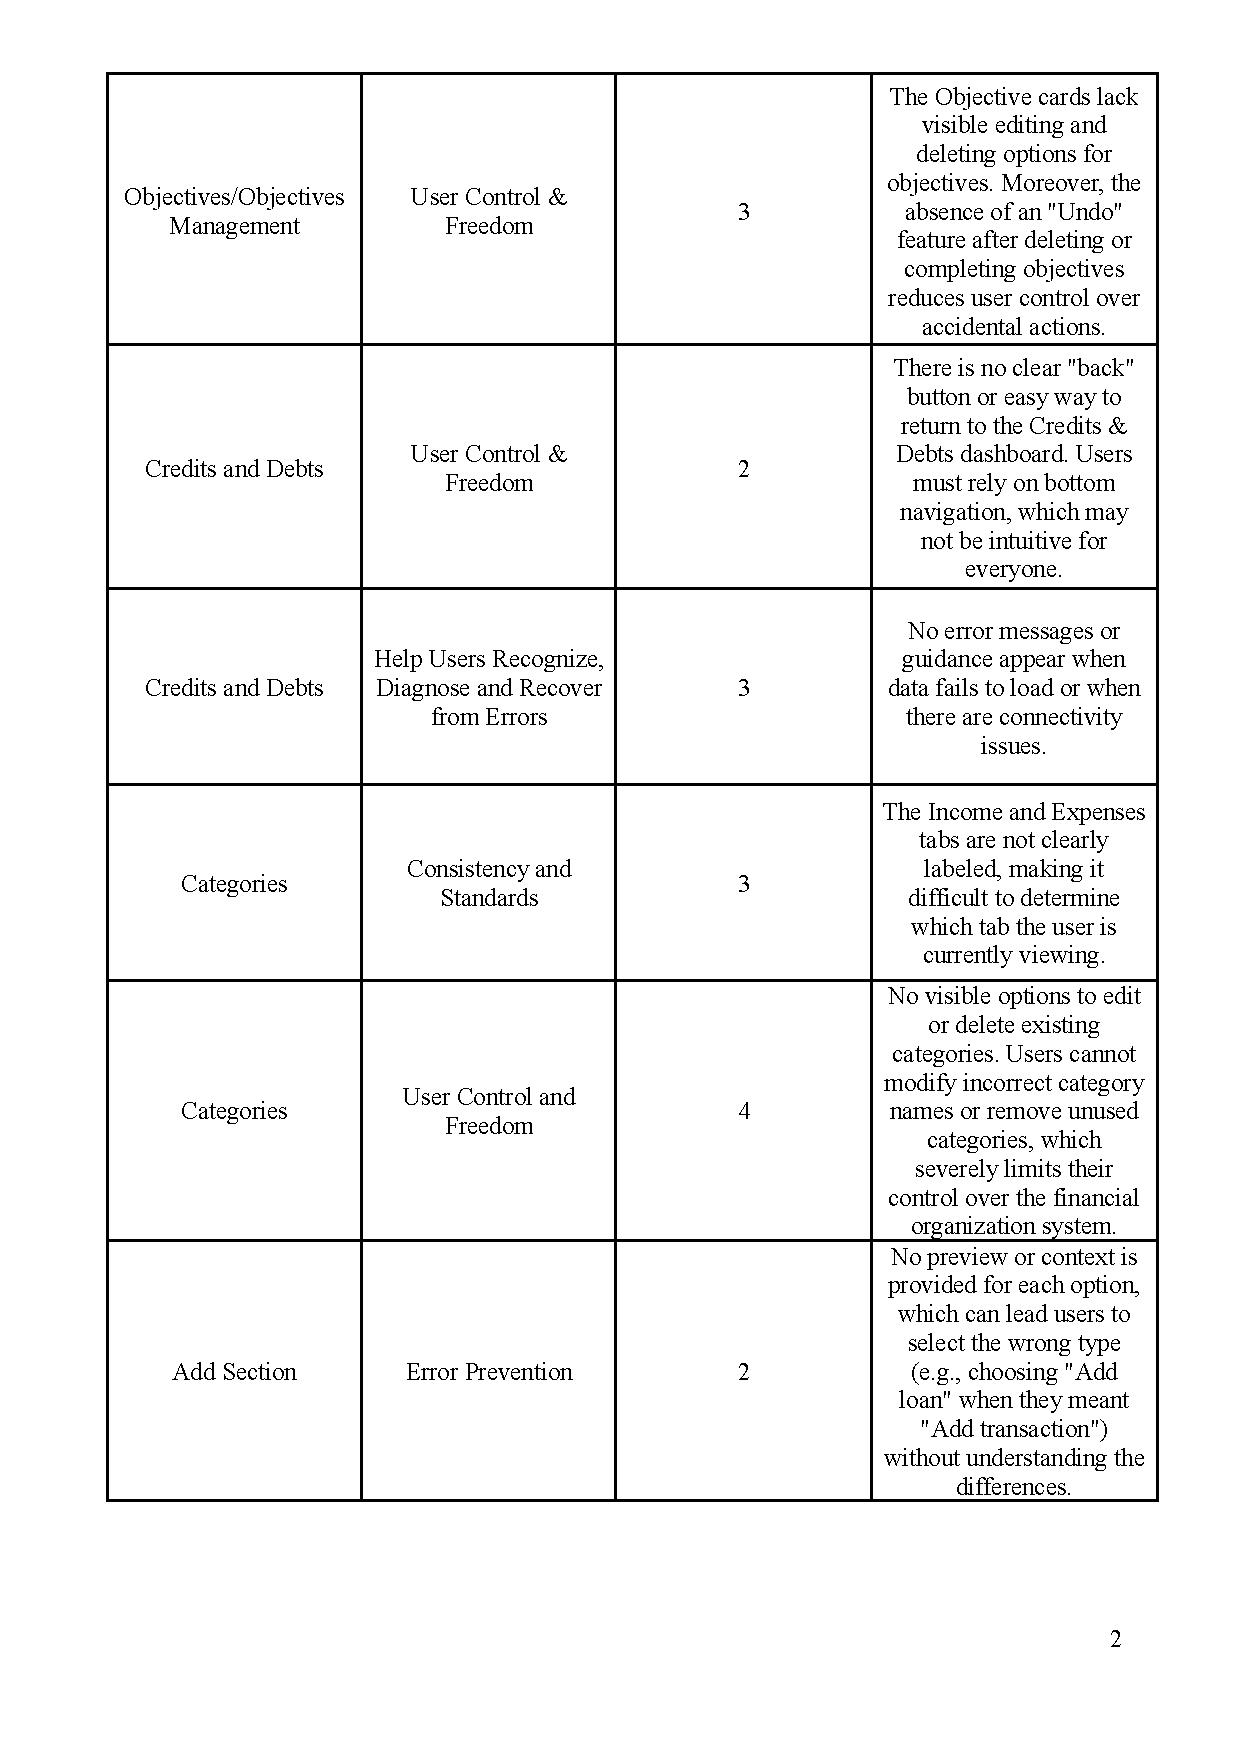
\includegraphics[width=1\linewidth]{HE2.pdf}
\end{figure}
\begin{figure}[H]
    \centering
    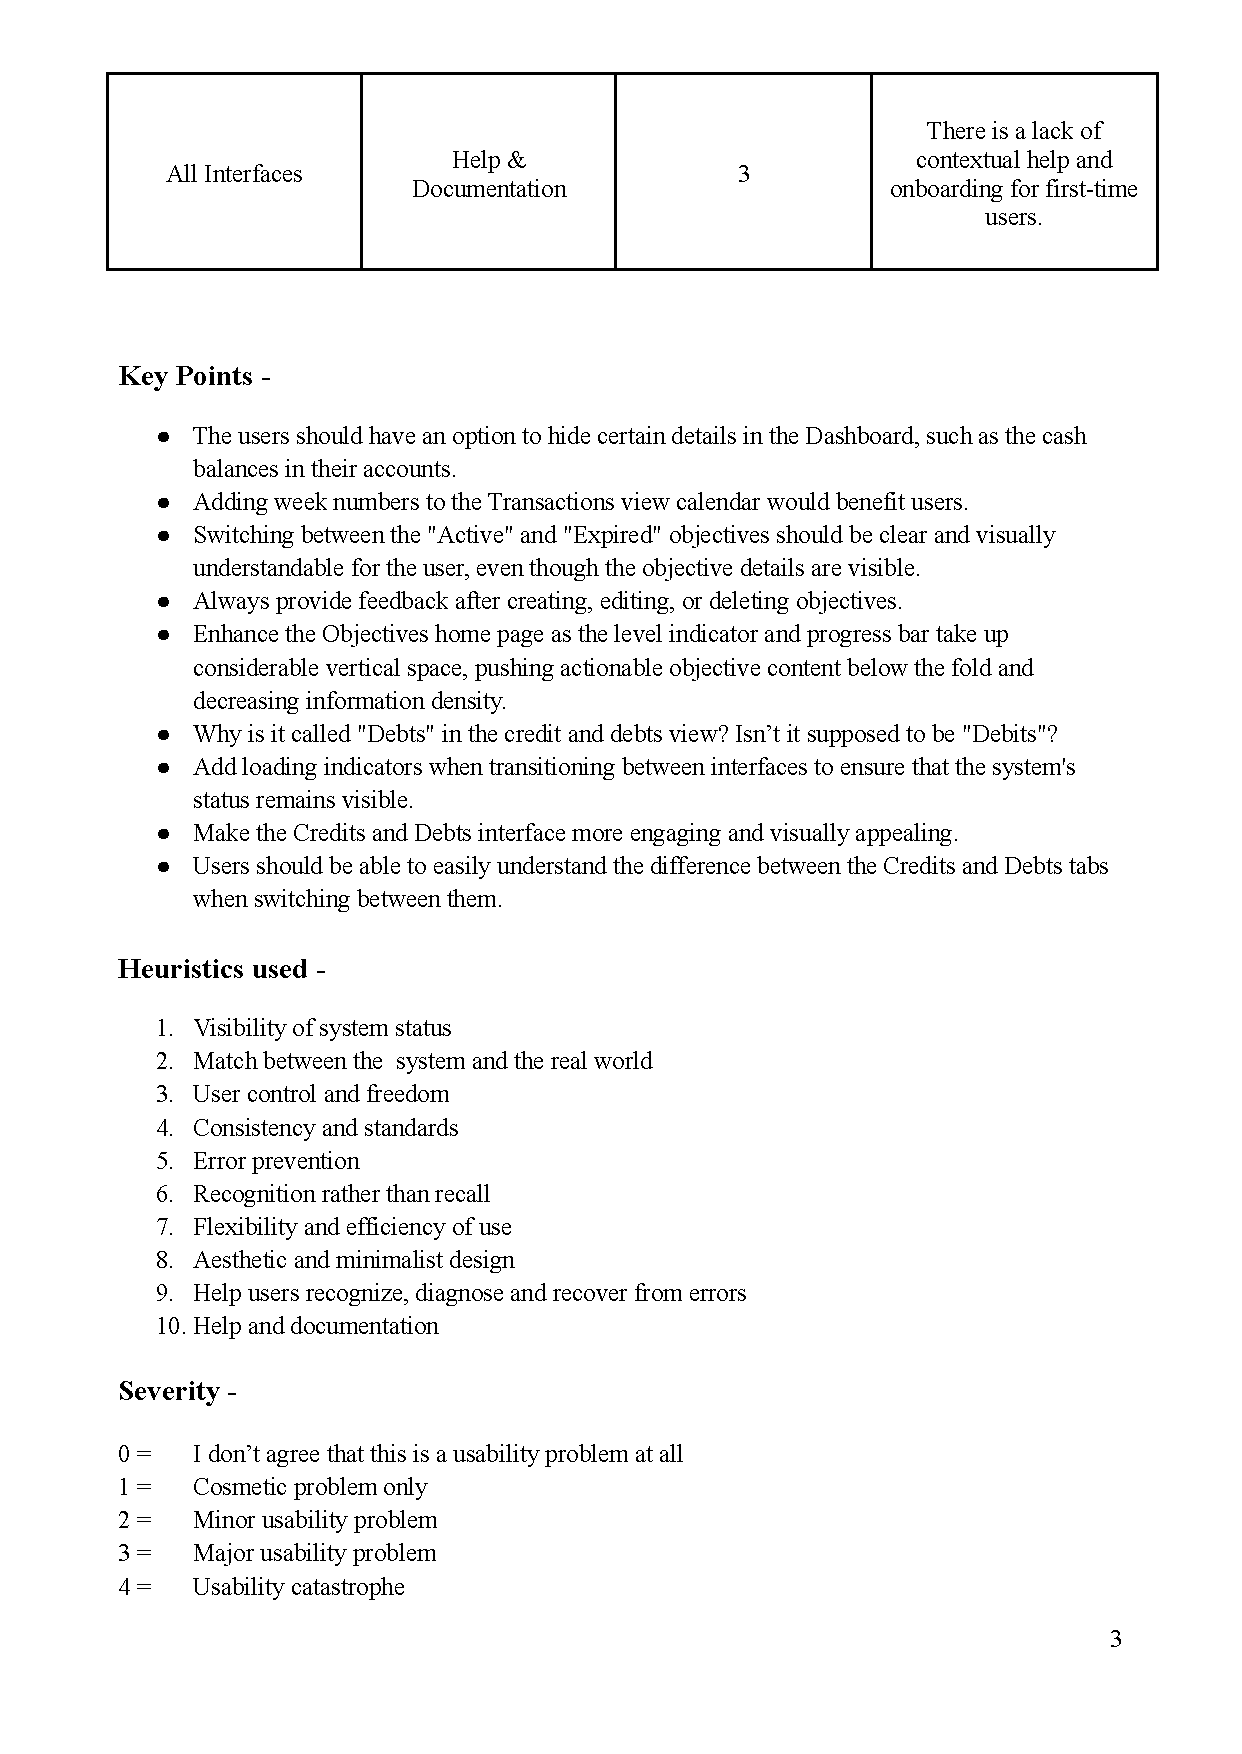
\includegraphics[width=1\linewidth]{HE3.pdf}
\end{figure}
\subsection{Prototype ONE}
After the Heuristic Evaluation we improved our interface by solving the problems raised by the experts. The prototype number ONE was created, a fully functional android app using Android Studio. Here are the fixes to some of the major usability problems highlighted in the Heuristic Evaluation:
\begin{itemize}
    \item The transactions screen now features an indication on the days that contain transactions
    \item Categories can be edited an deleted and it is clearly stated how to do so
    \item When selecting a day with no transactions, a message is displayed
    \item In several interfaces, there is now a message the informs the user of the functionality of said interface; this should help first-time users
\end{itemize}
\begin{figure}[H]
    \centering
    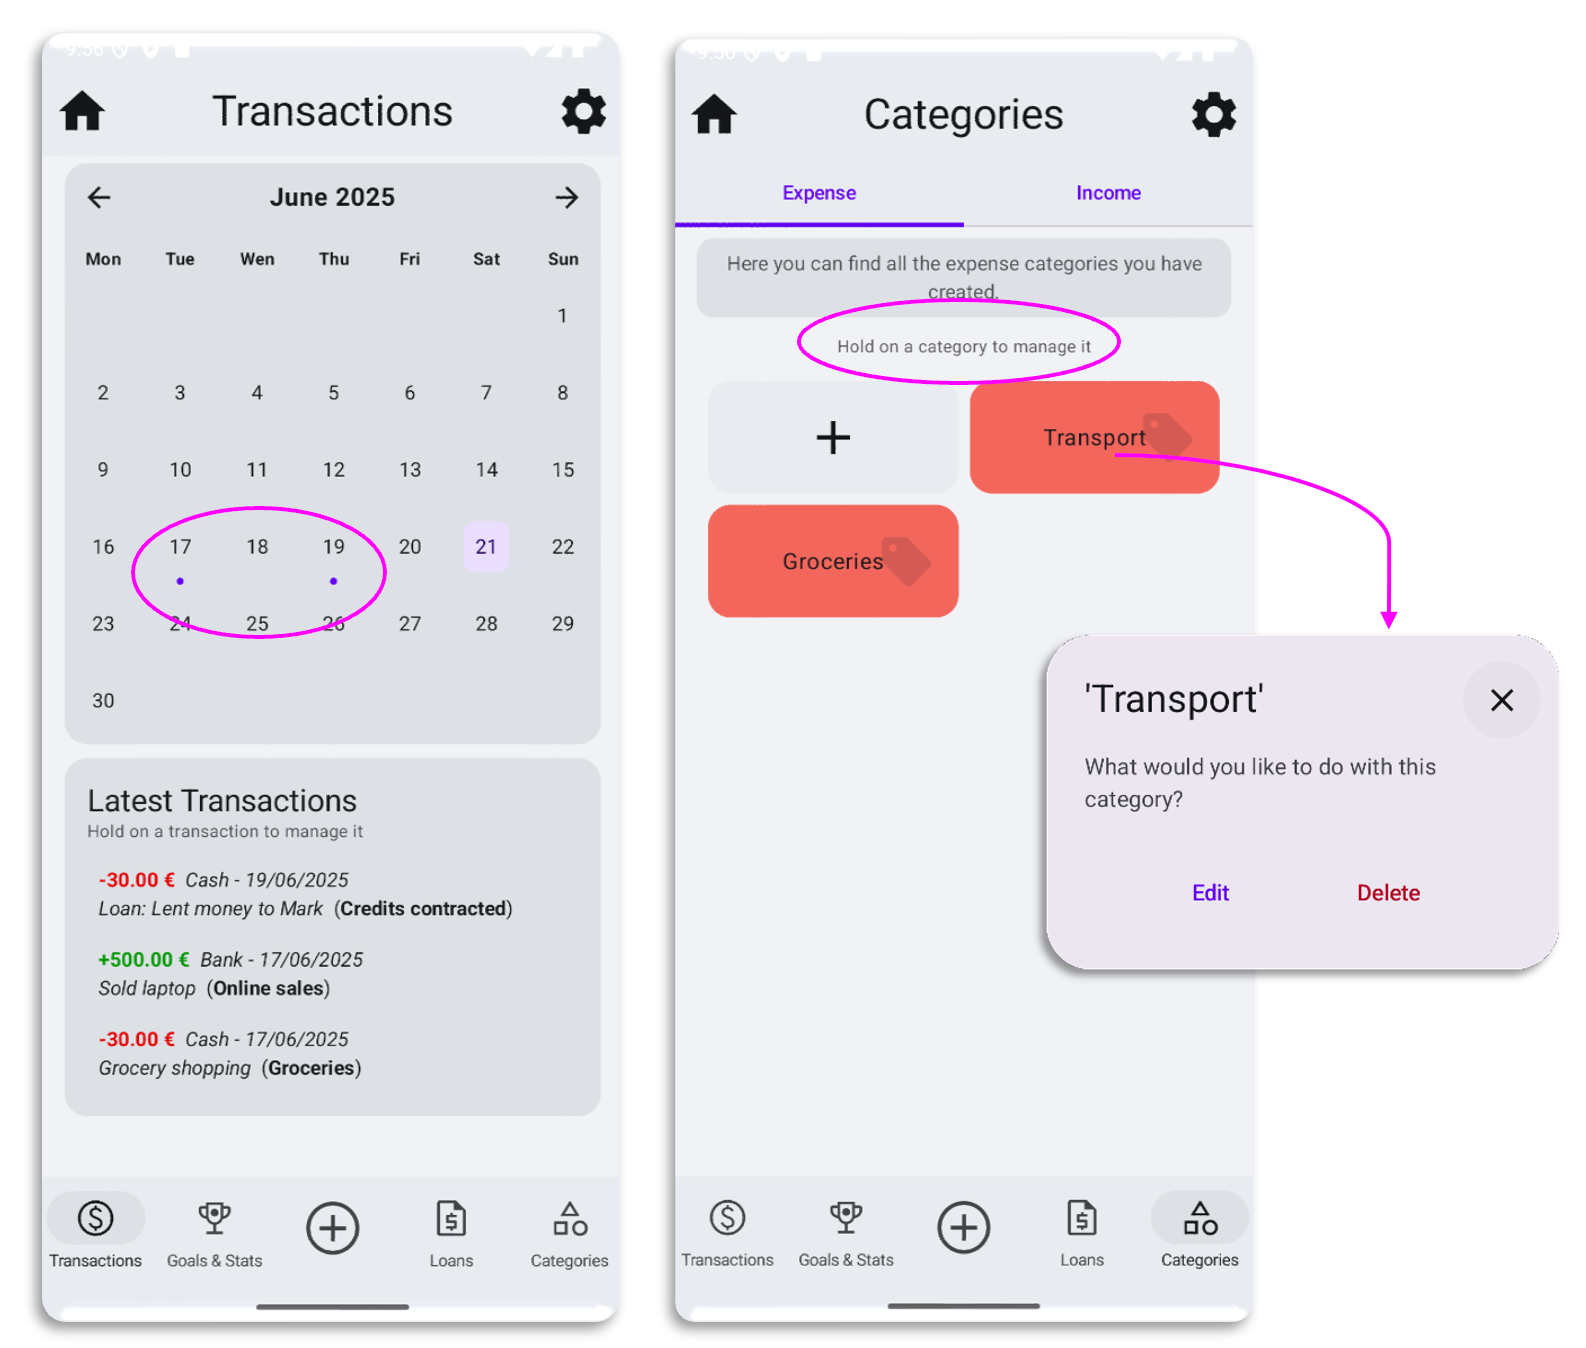
\includegraphics[scale=0.6]{HEres.png}
\end{figure}
\begin{figure}[H]
    \centering
    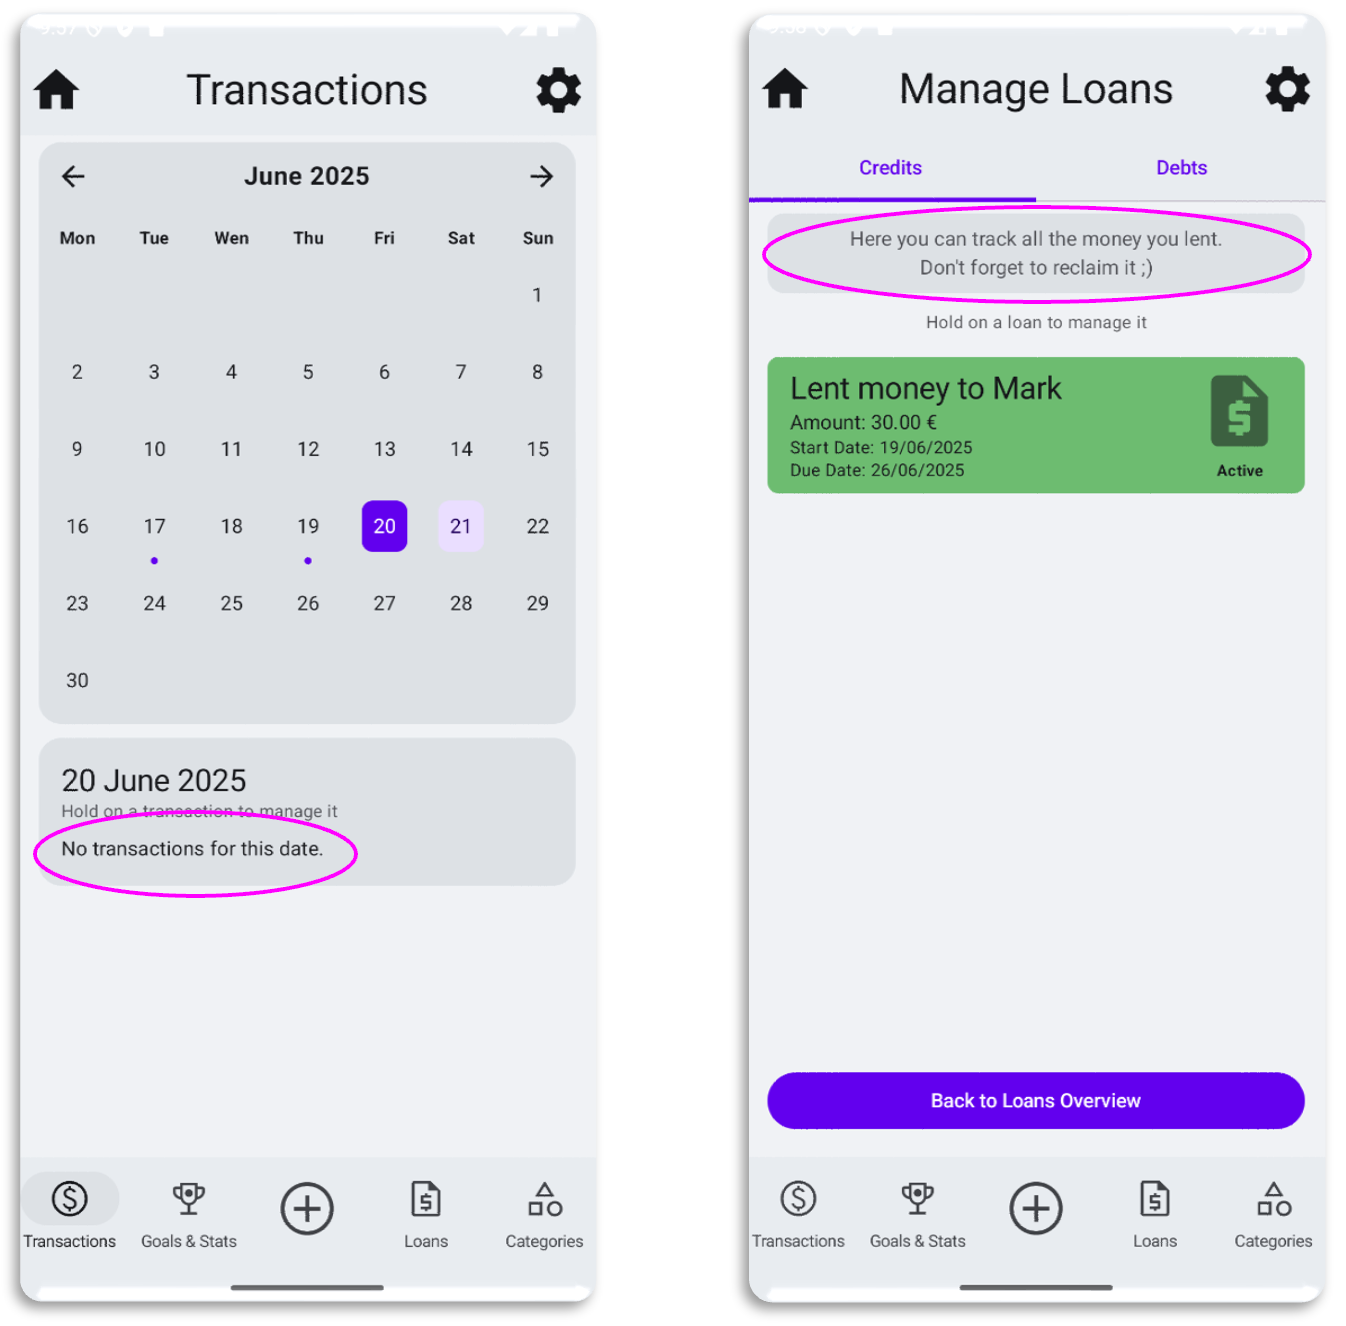
\includegraphics[scale=0.6]{HEres2.png}
\end{figure}
The other less severe problems were also promptly resolved, while some others only surfaced from the extreme simplicity of the mockups and were easily implemented in the realization.
\subsubsection{User Evaluation}
With the working application we tested it on a bunch of users by performing the "Think Aloud". We asked users to perform the following task:
\begin{itemize}
    \item Add a transaction
    \item Set a PIN for secure access
    \item Set a goal, mark it as reached and check your stats
\end{itemize}
The first two tasks were performed fairly easily. Thanks to the icons, the add button and the settings button were located quickly and from there the interaction continued as expected, with users inserting details for the addition of the transaction and for the setting of the PIN code.
\vspace{0.5cm}\\
However while conducting the evaluation of the third task, we noticed that users had trouble locating the stats page, which is in the same section as the goals.
Therefore, we decide to rename objectives to "goals" and to rename the Objectives section to "Goals \& Stats" to make it more clear.
While doing this we also added stats related to loans.
\begin{figure}[H]
    \centering
    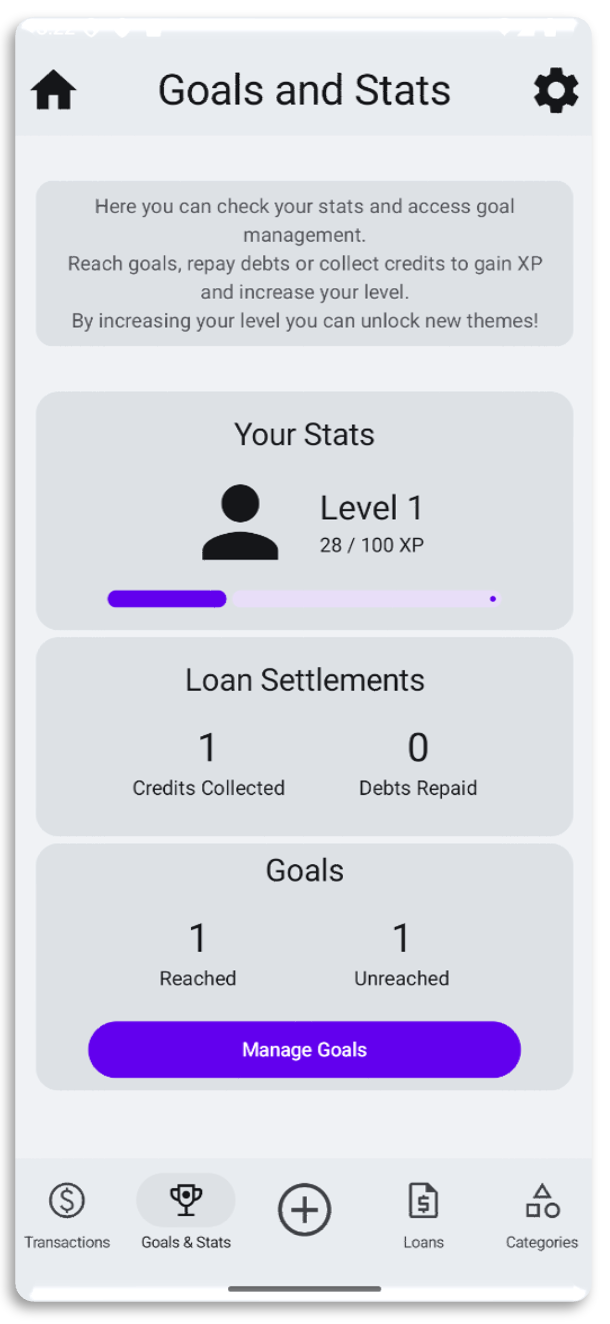
\includegraphics[scale=0.6]{G&T.png}
\end{figure}
\subsubsection{Controlled Experiment}
For the controlled experiment we designed two styles of interfaces for the navigation bar and the add dialog: one with labels and one with icons only. 
We divided users in two groups of 10 people each and tested each group on one of the two interfaces.\\The task the users were asked to perform was the following:
\vspace{0.5cm}\\
\textbf{Add a debt, then mark it as repaid and check your stats}
\vspace{0.5cm}\\
Hypothesis:
\begin{itemize}
    \item Null: no differences between the two interfaces
    \item Our: users will complete the task in less time using the interface with
    labels (interface A).
\end{itemize}
\begin{figure}[H]
    \centering
    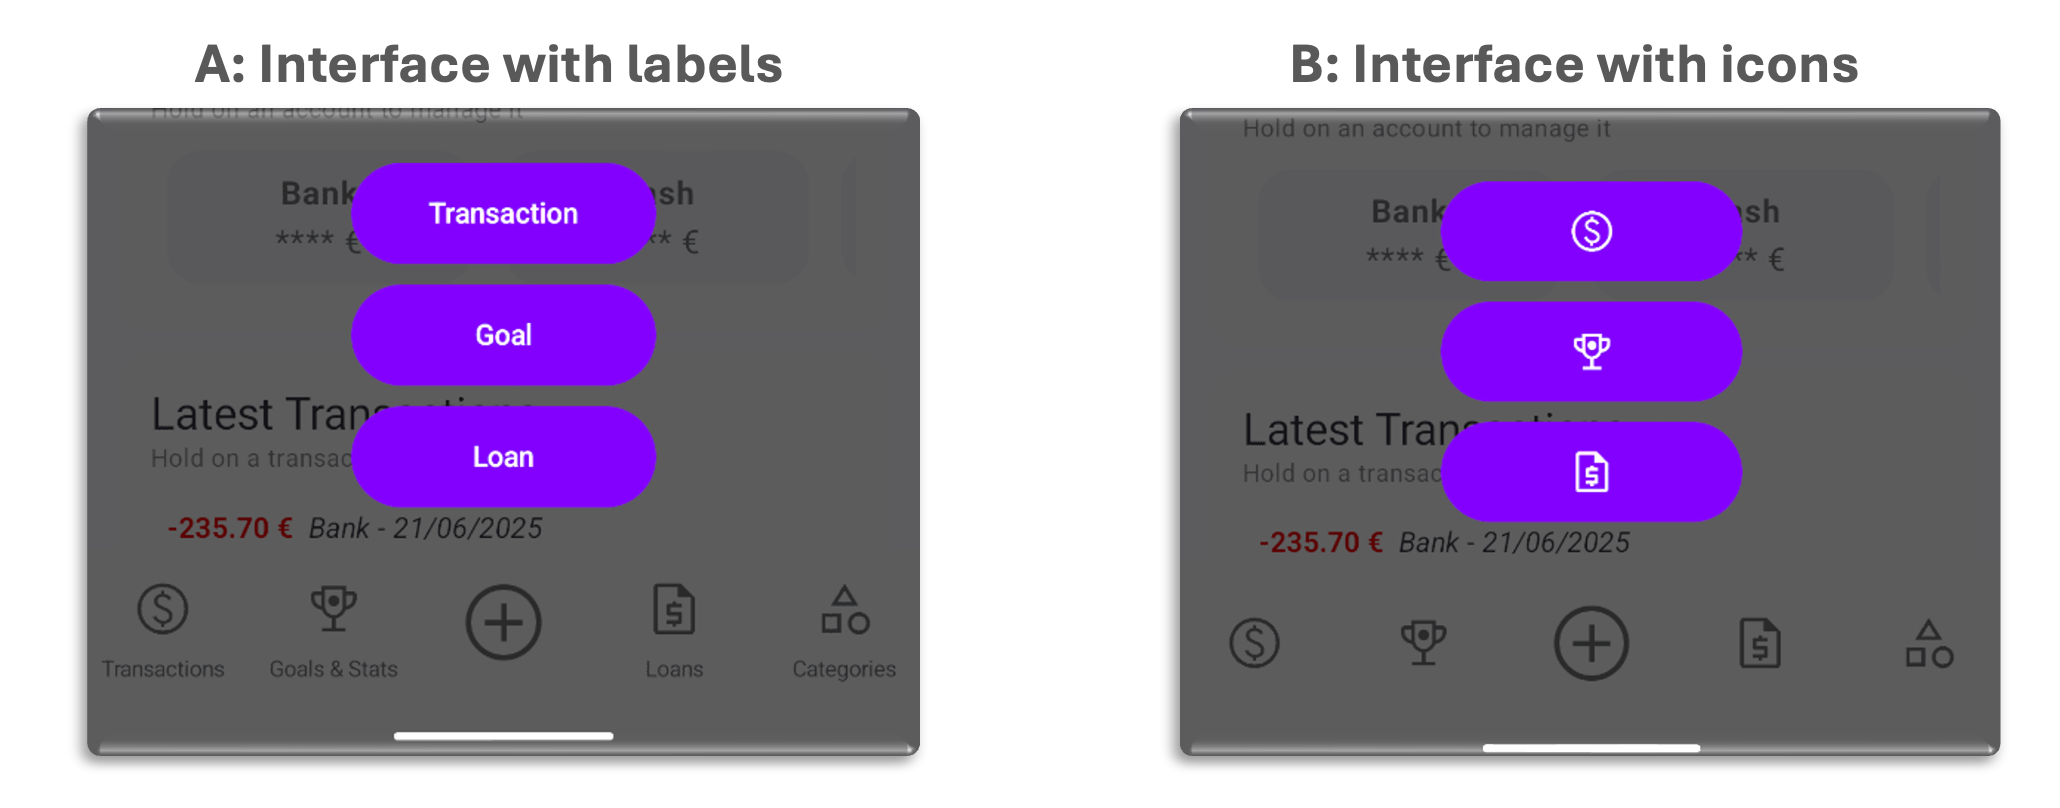
\includegraphics[width=\linewidth]{interf.png}
\end{figure}
We measured the time taken to complete the task for each user:
\begin{itemize}
    \item Group A: interface with labels
    \item Group B: interface with icons
\end{itemize}
\begin{figure}[H]
    \centering
    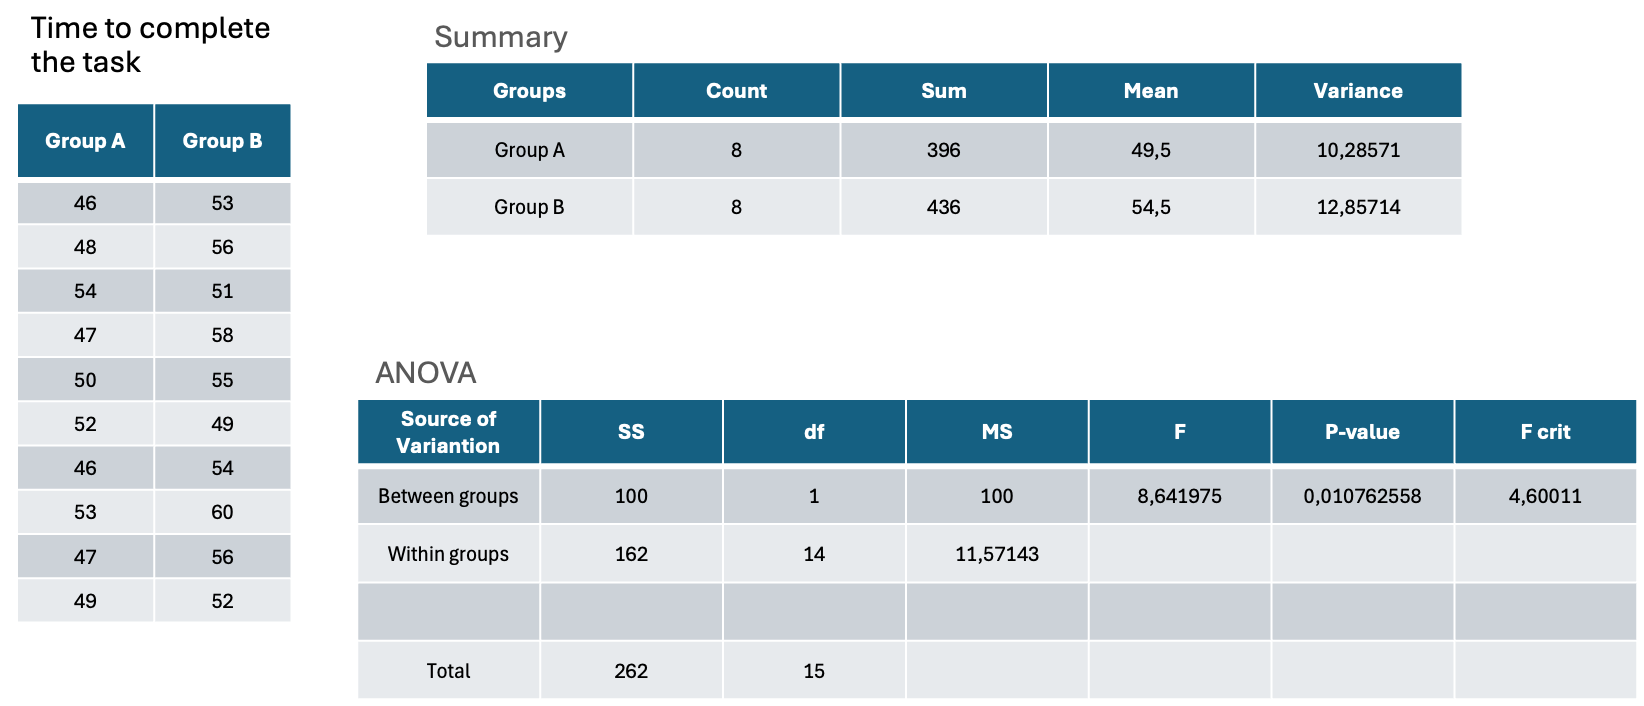
\includegraphics[width=\linewidth]{ANOVA.png}
\end{figure}
From the results of the ANOVA we can see that:\\
\[
F > F_{\text{crit}}
\]
meaning there is a statistically significant difference in task times between Group A and Group B. We can thus reject the null hypothesis and, by looking at the mean times to perform the task, conclude that the interface used by Group A (the one with labels) is better than the one used by Group B.\\
Therefore, we chose to use the interface with labels in the final prototype.

\subsection{Prototype TWO and FINAL}
Thanks to the help of our users and of the evaluations conducted by the team we were able to provide the second prototype and final version of our application.


\section{Final Realization}
\label{sec:final_realization}
This section presents the key screens of the final Budgify application, demonstrating its core functionalities and user interface design. The application aims to provide a comprehensive yet intuitive experience for personal finance management.

\subsection{Dashboard and Core Navigation}
The dashboard serves as the main entry point, offering an overview of finances. Navigation is facilitated by a bottom bar. Account management is also accessible from the dashboard, alongside chart visualization of transactions, including a switch between income and expenses and two types of charts. An account filter is also present to select which accounts to show in the charts.

\begin{figure}[H]
    \centering
    \begin{subfigure}[b]{0.23\textwidth}
        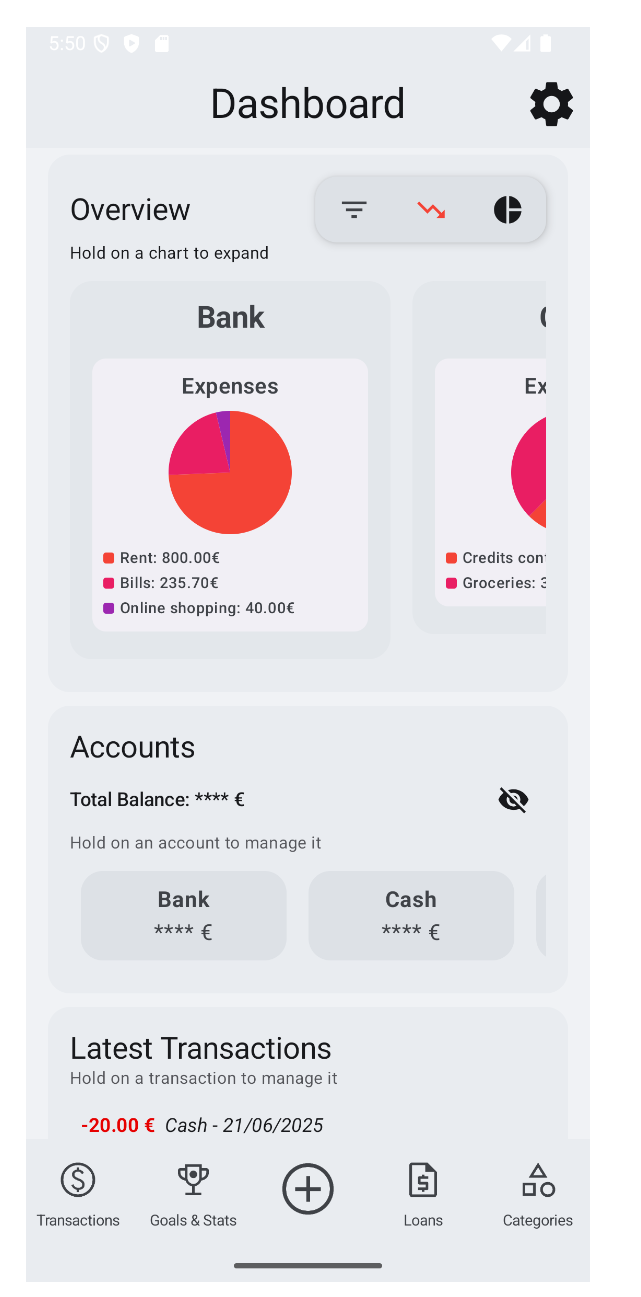
\includegraphics[width=\textwidth]{dashboard.png}
        \caption{Dashboard overview.}
        \label{fig:dashboard_overview}
    \end{subfigure}
    \hfill
    \begin{subfigure}[b]{0.23\textwidth}
        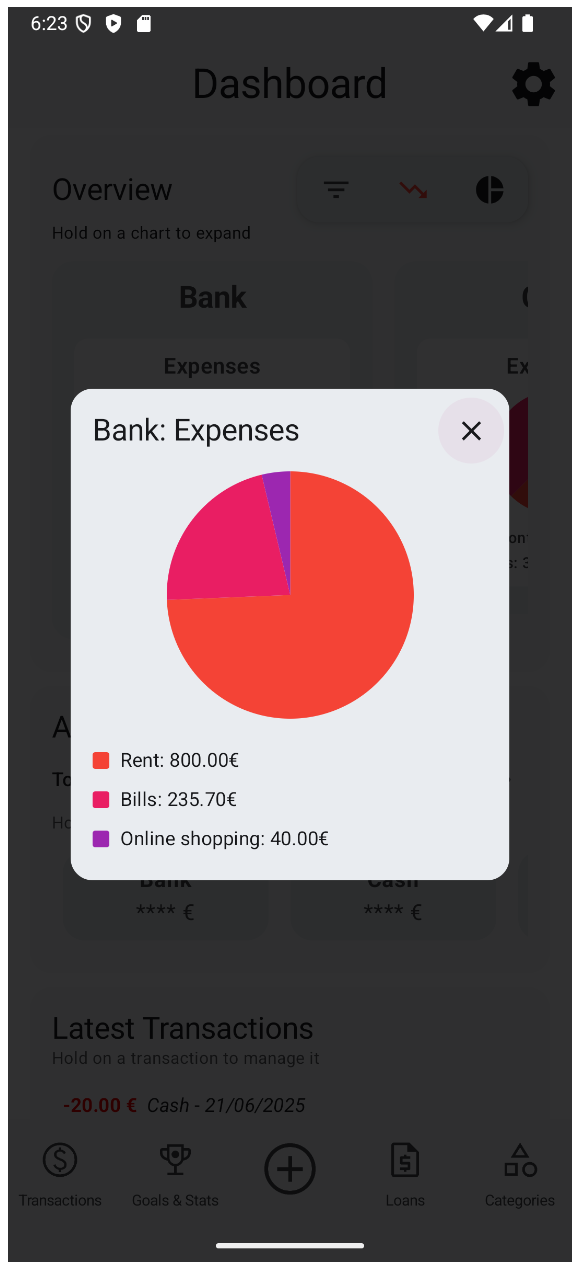
\includegraphics[width=\textwidth]{chart_dialog_pie.png}
        \caption{Expanded pie chart view.}
        \label{fig:dashboard_pie_expanded}
    \end{subfigure}
    \hfill
    \begin{subfigure}[b]{0.23\textwidth}
        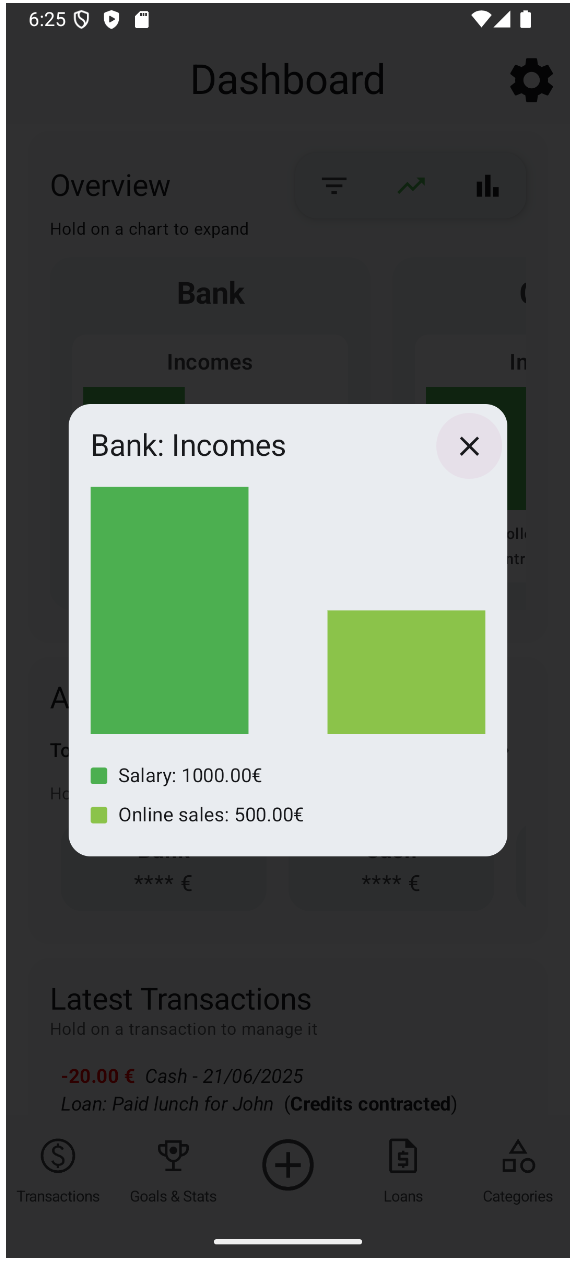
\includegraphics[width=\textwidth]{chart_dialog_histogram.png}
        \caption{Expanded bar chart view.}
        \label{fig:dashboard_bar_expanded}
    \end{subfigure}
    \hfill
    \begin{subfigure}[b]{0.23\textwidth}
        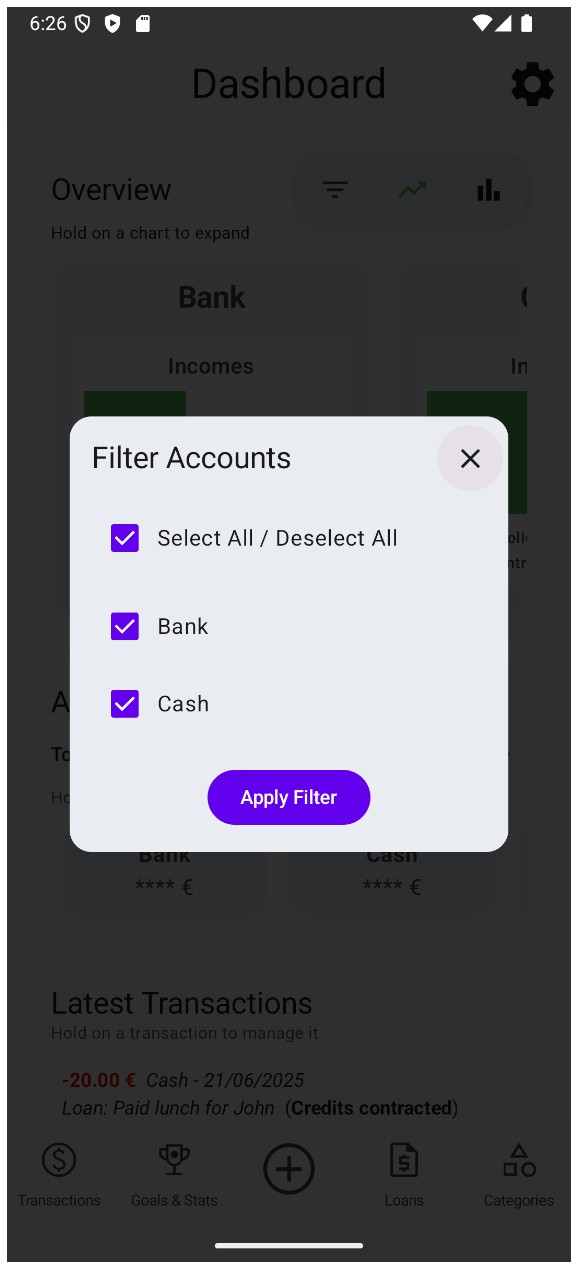
\includegraphics[width=\textwidth]{chart_dialog_filter.png}
        \caption{Filtering accounts for dashboard view.}
        \label{fig:dashboard_filter_accounts}
    \end{subfigure}
    \caption{Dashboard views and initial interactions.}
    \label{fig:dashboard_interactions}
\end{figure}

\begin{figure}[H]
    \centering
    \begin{subfigure}[b]{0.23\textwidth}
        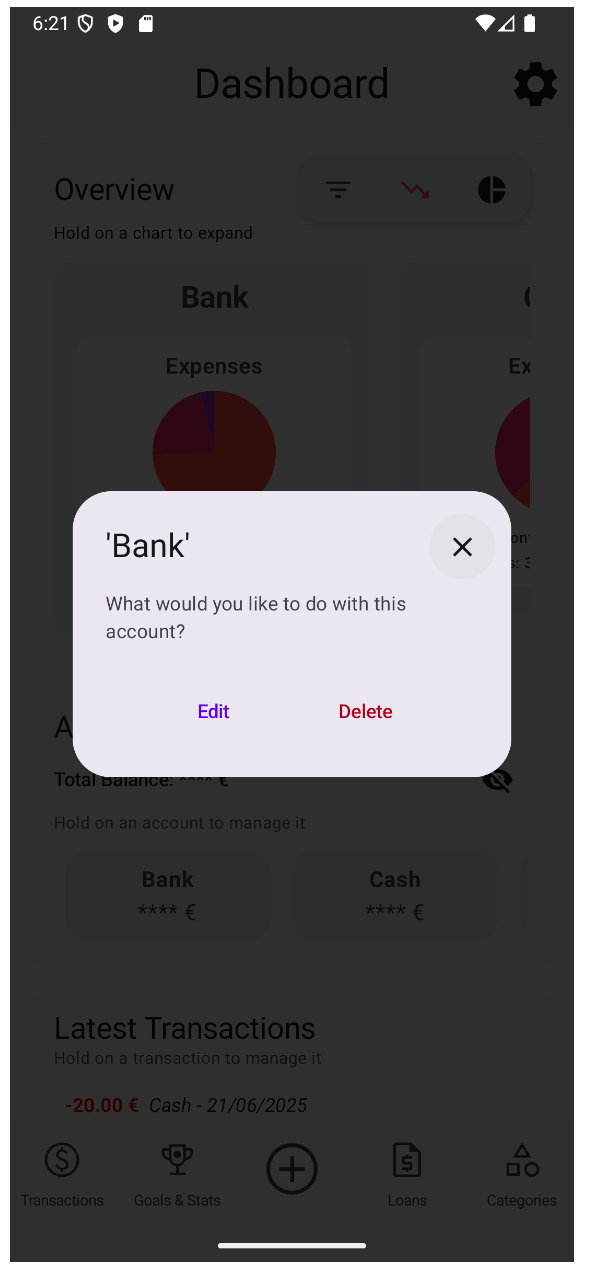
\includegraphics[width=\textwidth]{account_interaction_dialog.png}
        \caption{Account actions: Edit/Delete.}
        \label{fig:dashboard_account_actions}
    \end{subfigure}
    \hfill
    \begin{subfigure}[b]{0.23\textwidth}
        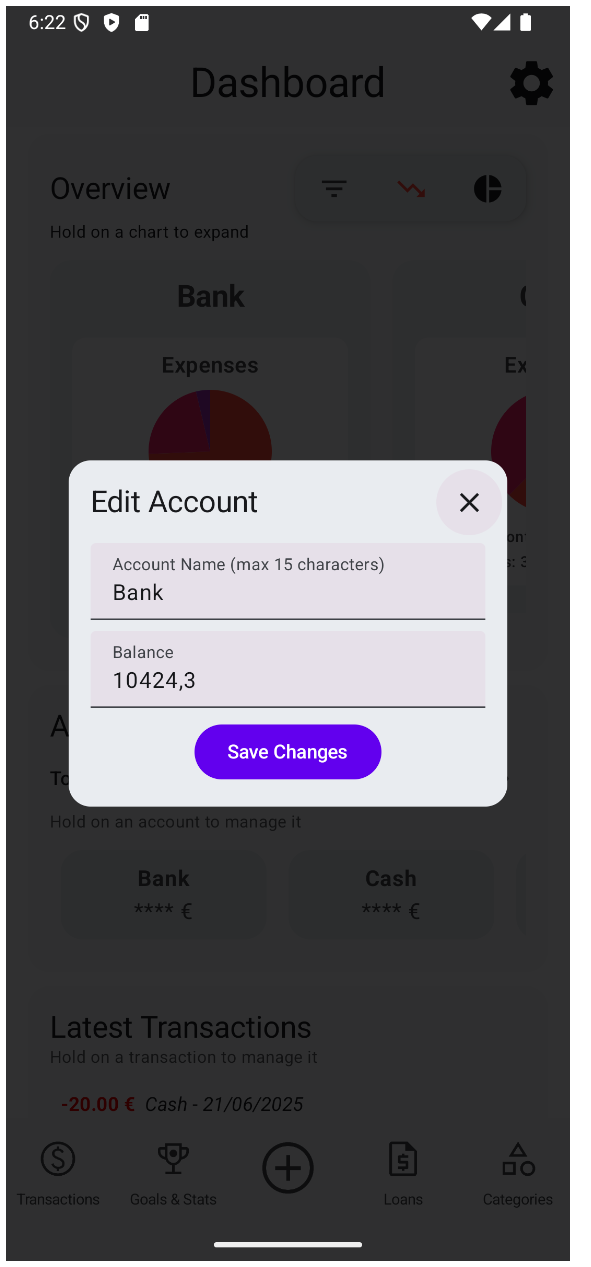
\includegraphics[width=\textwidth]{account_edit_dialog.png}
        \caption{Editing an account's details.}
        \label{fig:dashboard_edit_account}
    \end{subfigure}
    \hfill
    \begin{subfigure}[b]{0.23\textwidth}
        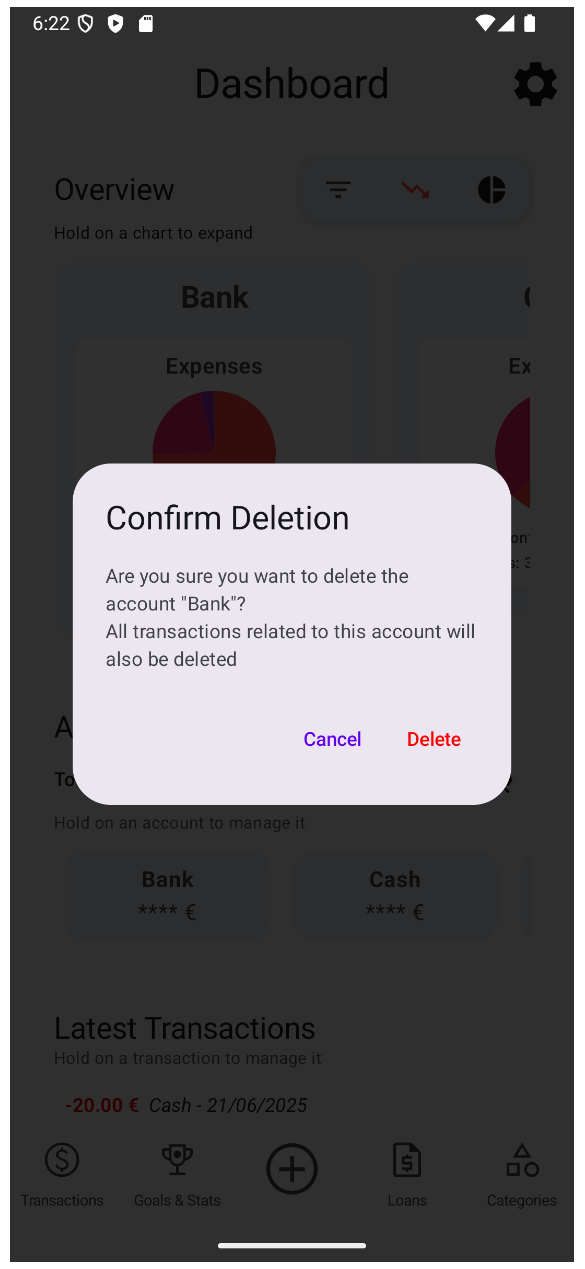
\includegraphics[width=\textwidth]{account_deletion_dialog.png}
        \caption{Confirming account deletion.}
        \label{fig:dashboard_delete_account_confirm}
    \end{subfigure}
    \caption{Managing accounts from the dashboard.}
    \label{fig:dashboard_account_management}
\end{figure}

\subsection{Adding New Entries (Transaction, Goal, Loan)}
A central "+" button provides access to adding new transactions, goals, or loans.

\begin{figure}[H]
    \centering
    \begin{subfigure}[b]{0.23\textwidth}
        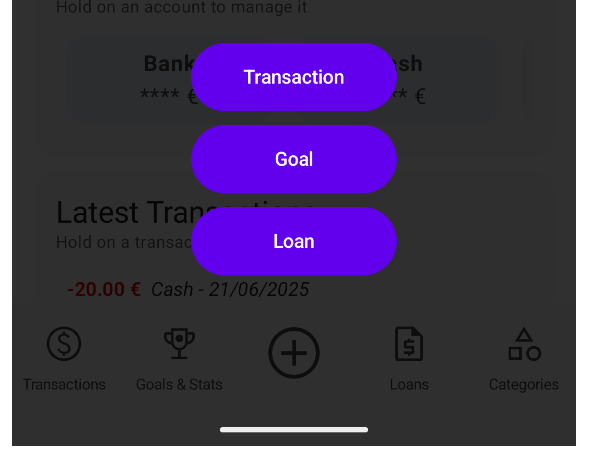
\includegraphics[width=\textwidth]{add_dialog.png}
        \caption{Options after tapping the add button.}
        \label{fig:add_options}
    \end{subfigure}
    \hfill
    \begin{subfigure}[b]{0.23\textwidth}
        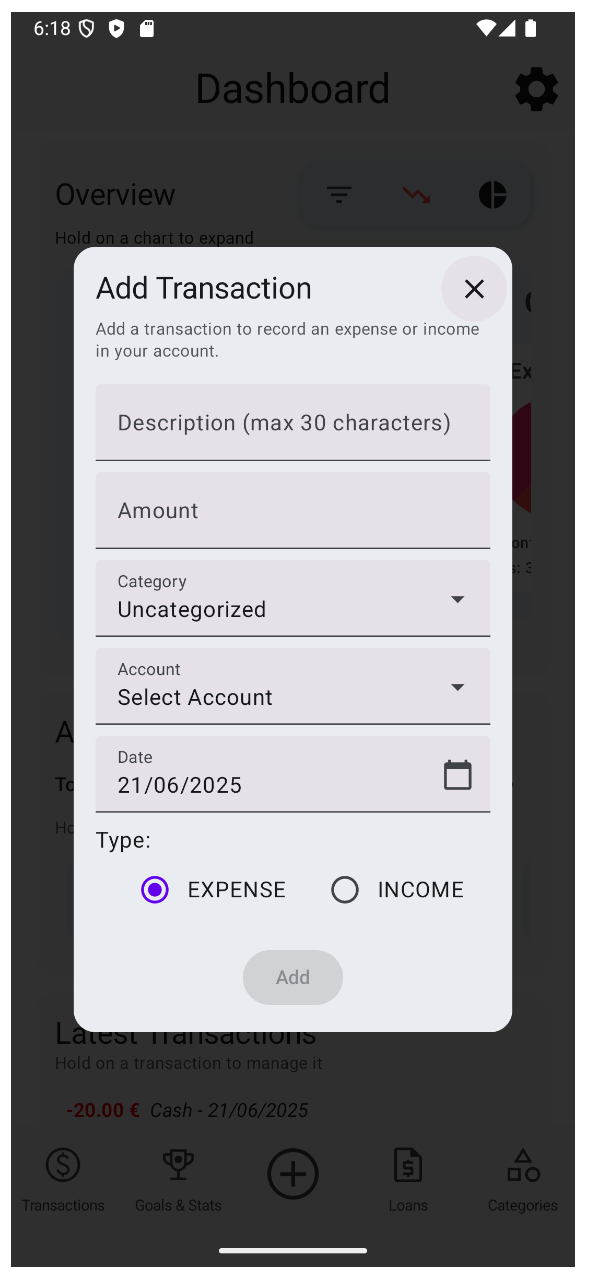
\includegraphics[width=\textwidth]{add_transaction_dialog.png}
        \caption{Form for adding a new transaction.}
        \label{fig:add_transaction_form}
    \end{subfigure}
    \hfill
    \begin{subfigure}[b]{0.23\textwidth}
        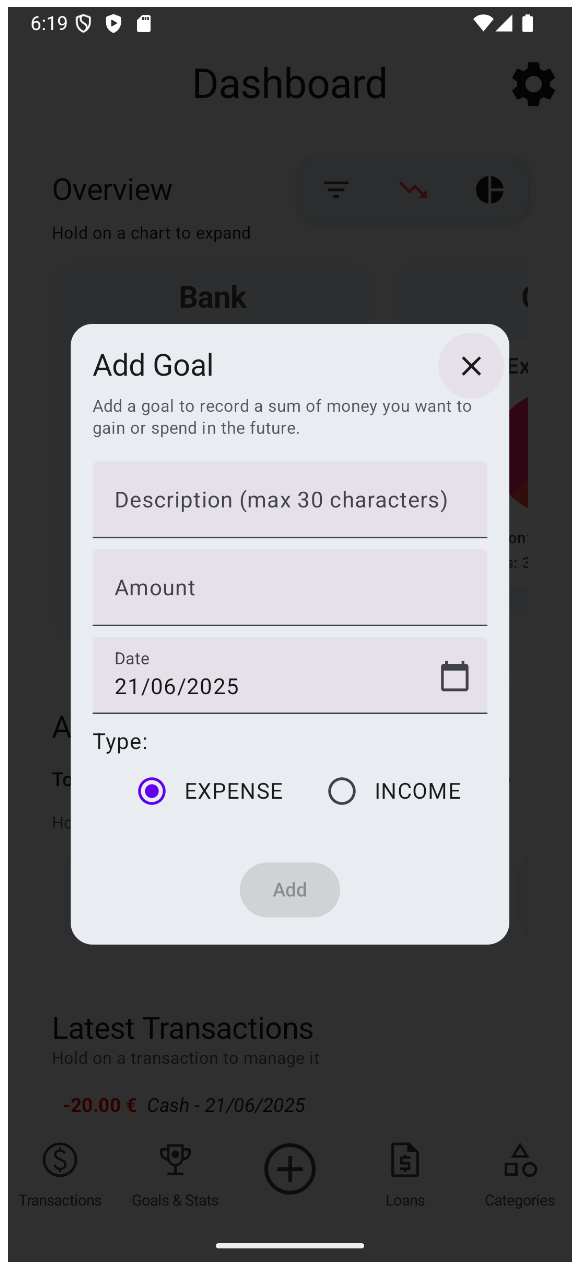
\includegraphics[width=\textwidth]{add_goal_dialog.png}
        \caption{Form for adding a new financial goal.}
        \label{fig:add_goal_form}
    \end{subfigure}
    \hfill
    \begin{subfigure}[b]{0.23\textwidth}
        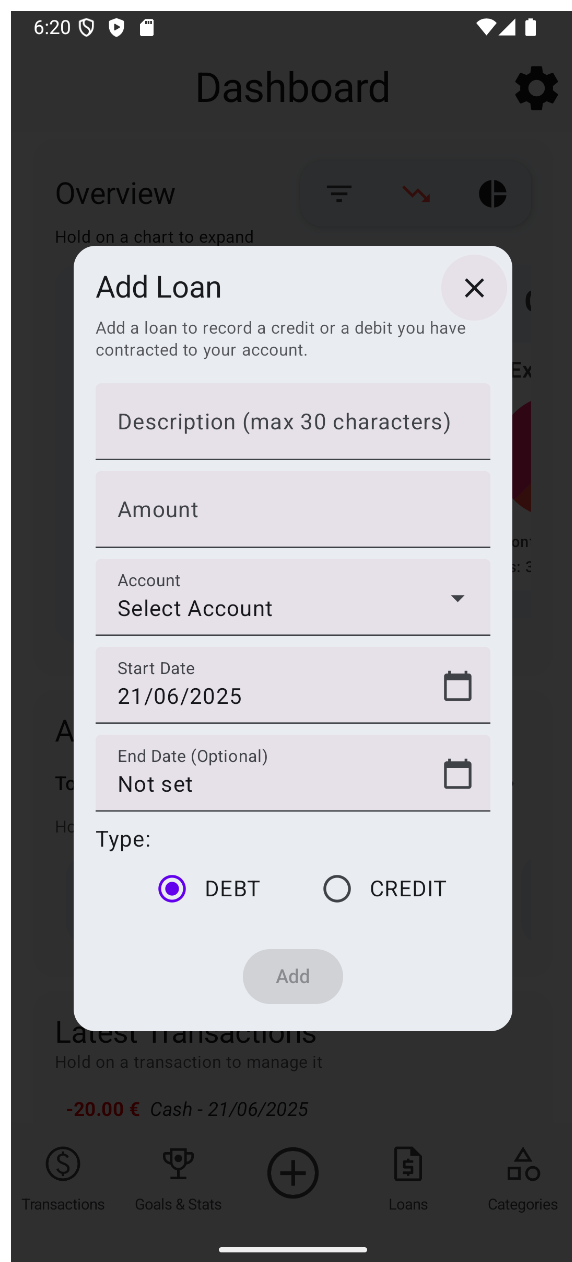
\includegraphics[width=\textwidth]{add_loan_dialog.png}
        \caption{Form for adding a new loan/debt.}
        \label{fig:add_loan_form}
    \end{subfigure}
    \caption{Adding new financial entries.}
    \label{fig:adding_entries}
\end{figure}

\subsection{Transaction Management}
Users can view transactions by day with the help of a calendar or as a list of latest transactions, and manage them individually.

\begin{figure}[H]
    \centering
    \begin{subfigure}[b]{0.23\textwidth}
        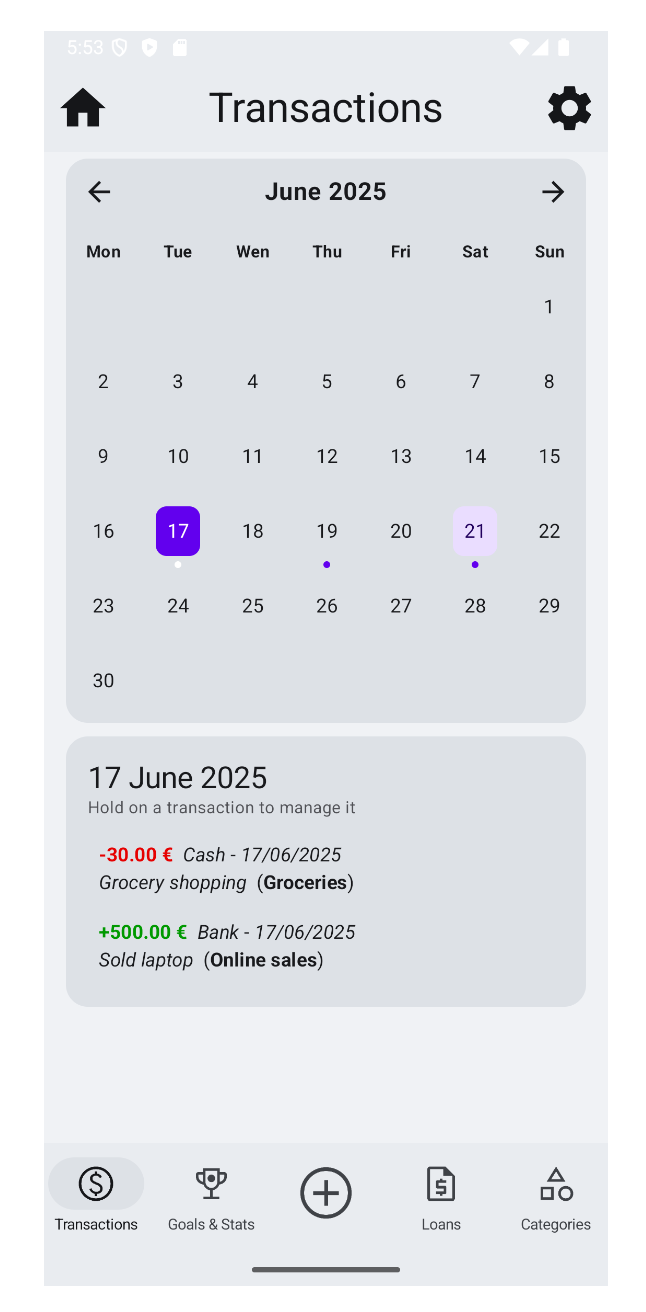
\includegraphics[width=\textwidth]{transactions_day.png}
        \caption{Transactions for a specific day (e.g., 17 June 2025).}
        \label{fig:transactions_specific_day}
    \end{subfigure}
    \hfill
    \begin{subfigure}[b]{0.23\textwidth}
        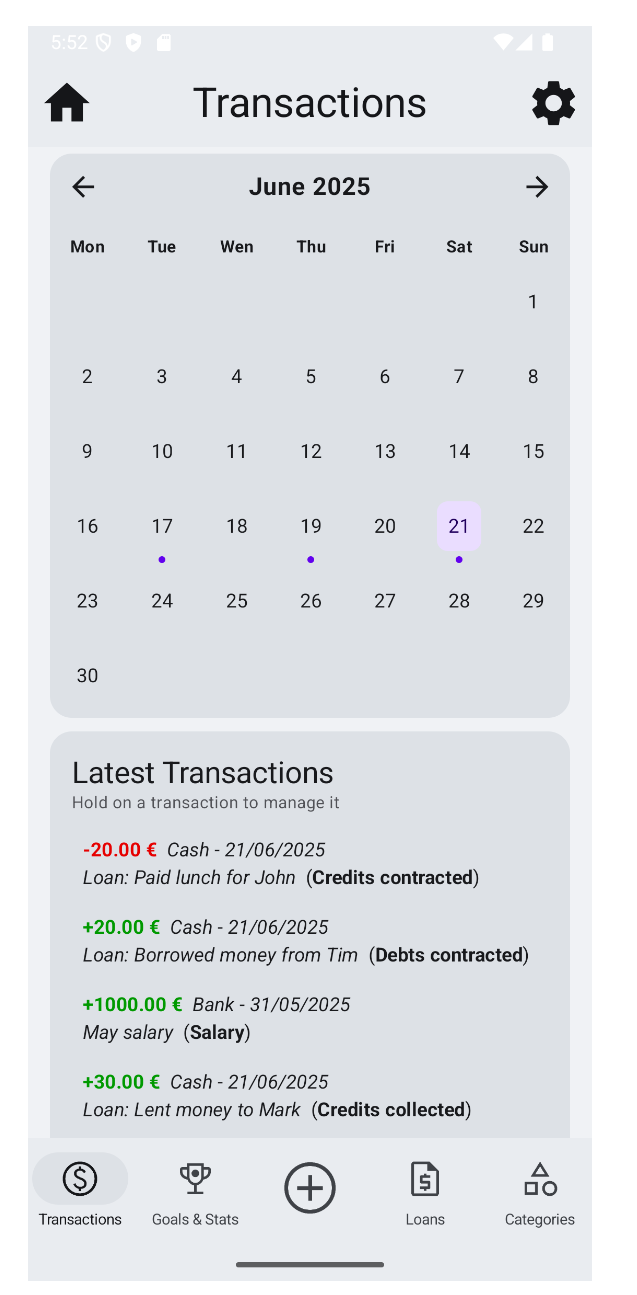
\includegraphics[width=\textwidth]{transactions.png}
        \caption{List of latest transactions (default view).}
        \label{fig:transactions_latest}
    \end{subfigure}
    \hfill
    \begin{subfigure}[b]{0.23\textwidth}
        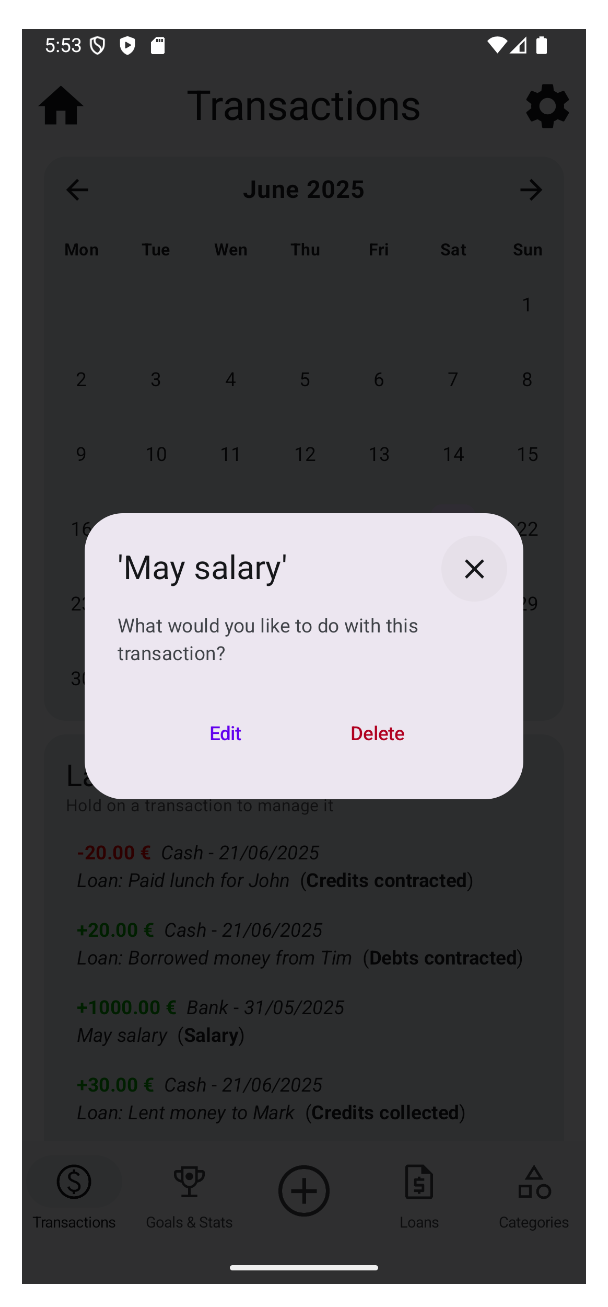
\includegraphics[width=\textwidth]{transactions_interaction_dialog.png}
        \caption{Transaction dialog interaction.}
        \label{fig:transaction_edit_delete_dialog}
    \end{subfigure}
    \hfill
    \begin{subfigure}[b]{0.23\textwidth}
        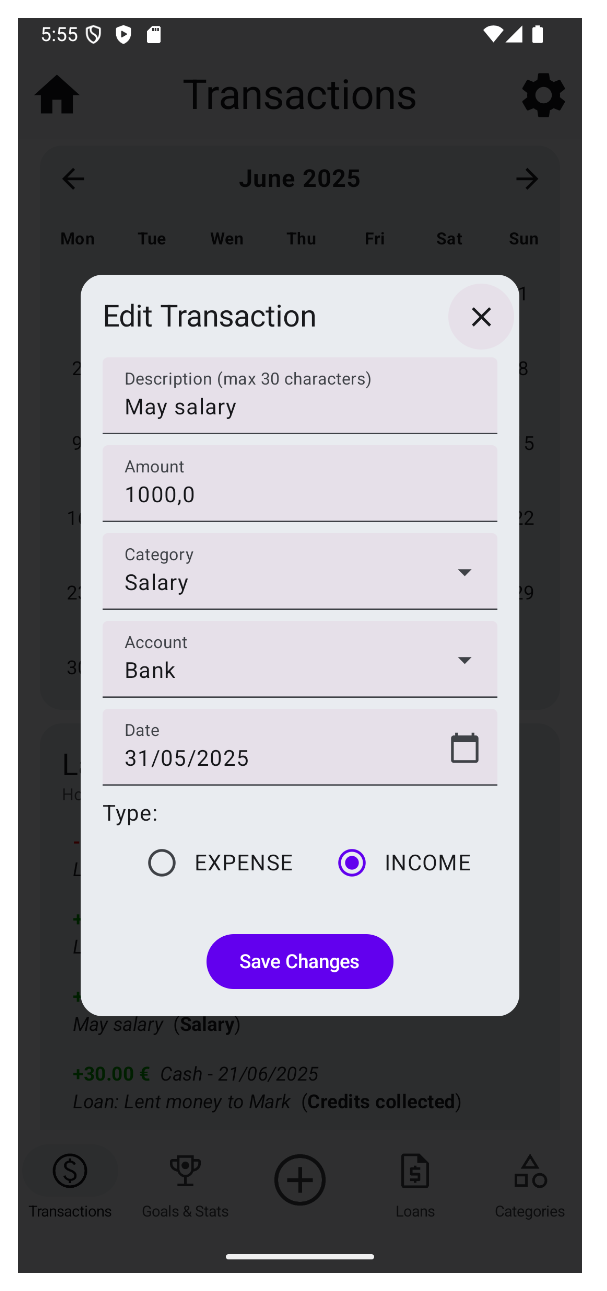
\includegraphics[width=\textwidth]{transactions_edit_dialog.png}
        \caption{Editing transaction details.}
        \label{fig:transaction_edit_form}
    \end{subfigure}
    \par\bigskip % A little vertical space before the next subfigure if needed
    \begin{subfigure}[b]{0.23\textwidth}
        \includegraphics[width=\textwidth]{transactions_delete_dialog.png}
        \caption{Confirming transaction deletion.}
        \label{fig:transaction_delete_confirm}
    \end{subfigure}
    \caption{Transaction viewing and management.}
    \label{fig:transaction_management}
\end{figure}
\vspace{1cm}
\subsection{Goals and Stats}
This section allows users to track their financial goals and view overall statistics, including number of goals reached, credits collected and debts repaid. The user's overall level is also displayed here. To increase their level, the user can reach goals, repay debts or collect credits. After reaching a certain level, a reward can be unlocked.

\begin{figure}[H]
    \centering
    \begin{subfigure}[b]{0.23\textwidth}
        \includegraphics[width=\textwidth]{goals_stats.png}
        \caption{Goals and Stats overview page with user level and summaries.}
        \label{fig:goals_stats_overview}
    \end{subfigure}
    \hfill
    \begin{subfigure}[b]{0.23\textwidth}
        \includegraphics[width=\textwidth]{manage_goals_active.png}
        \caption{Managing active goals (e.g., 'Save money', 'New game').}
        \label{fig:manage_goals_active}
    \end{subfigure}
    \hfill
    \begin{subfigure}[b]{0.23\textwidth}
        \includegraphics[width=\textwidth]{manage_goals_inactive.png}
        \caption{Viewing inactive/reached goals (e.g., 'Shoes').}
        \label{fig:manage_goals_inactive}
    \end{subfigure}
    \hfill
    \begin{subfigure}[b]{0.23\textwidth}
        \includegraphics[width=\textwidth]{manage_goals_interaction_dialog.png}
        \caption{Dialog to Edit/Delete/Mark as Reached for a goal.}
        \label{fig:goal_actions_dialog}
    \end{subfigure}
    \caption{Goals and Statistics tracking.}
    \label{fig:goals_stats_tracking_1}
\end{figure}

\begin{figure}[H]
    \centering
    \ContinuedFloat % If this figure continues the previous one conceptually
    \begin{subfigure}[b]{0.23\textwidth}
        \includegraphics[width=\textwidth]{manage_goals_edit_dialog.png}
        \caption{Editing goal details.}
        \label{fig:goal_edit_form}
    \end{subfigure}
    \hfill
    \begin{subfigure}[b]{0.23\textwidth}
        \includegraphics[width=\textwidth]{manage_goals_delete_dialog.png}
        \caption{Confirming goal deletion.}
        \label{fig:goal_delete_confirm}
    \end{subfigure}
    \hfill
    \begin{subfigure}[b]{0.23\textwidth}
        \includegraphics[width=\textwidth]{manage_goals_complete_dialog.png}
        \caption{Selecting an account when marking a goal as reached.}
        \label{fig:goal_mark_reached_account}
    \end{subfigure}
    \caption{Managing individual goals (continued).}
    \label{fig:goals_stats_tracking_2}
\end{figure}

\subsection{Loan Management}
Budgify allows tracking of both money lent (credits) and borrowed (debts) through the loans section.

\begin{figure}[H]
    \centering
    \begin{subfigure}[b]{0.23\textwidth}
        \includegraphics[width=\textwidth]{loans.png}
        \caption{Loans overview showing total active credits and debts.}
        \label{fig:loans_overview}
    \end{subfigure}
    \hfill
    \begin{subfigure}[b]{0.23\textwidth}
        \includegraphics[width=\textwidth]{manage_loans_credits.png}
        \caption{Managing credits (money lent), e.g., 'Paid lunch for John'.}
        \label{fig:manage_credits}
    \end{subfigure}
    \hfill
    \begin{subfigure}[b]{0.23\textwidth}
        \includegraphics[width=\textwidth]{manage_loans_debts.png}
        \caption{Managing debts (money borrowed), e.g., 'Borrowed money from Tim'.}
        \label{fig:manage_debts}
    \end{subfigure}
    \hfill
    \begin{subfigure}[b]{0.23\textwidth}
        \includegraphics[width=\textwidth]{manage_loans_interaction_dialog.png}
        \caption{Dialog for loan actions: Edit/Delete/Mark as Collected.}
        \label{fig:loan_actions_dialog}
    \end{subfigure}
    \caption{Loan (Credits and Debts) management.}
    \label{fig:loan_management_1}
\end{figure}

\begin{figure}[H]
    \centering
    \ContinuedFloat
    \begin{subfigure}[b]{0.23\textwidth}
        \includegraphics[width=\textwidth]{manage_loans_edit_dialog.png}
        \caption{Editing loan/credit details.}
        \label{fig:loan_edit_form}
    \end{subfigure}
    \hfill
    \begin{subfigure}[b]{0.23\textwidth}
        \includegraphics[width=\textwidth]{manage_loans_delete_dialog.png}
        \caption{Confirming loan deletion.}
        \label{fig:loan_delete_confirm}
    \end{subfigure}
    \hfill
    \begin{subfigure}[b]{0.23\textwidth}
        \includegraphics[width=\textwidth]{manage_loans_complete_dialog.png}
        \caption{Selecting an account when marking a credit as collected.}
        \label{fig:loan_mark_collected_account}
    \end{subfigure}
    \caption{Managing individual loans/credits (continued).}
    \label{fig:loan_management_2}
\end{figure}

\subsection{Category Management}
Users can define and manage custom categories for both income and expenses.

\begin{figure}[H]
    \centering
    \begin{subfigure}[b]{0.23\textwidth}
        \includegraphics[width=\textwidth]{categories_expense.png}
        \caption{Managing expense categories (e.g., 'Transport').}
        \label{fig:categories_expense}
    \end{subfigure}
    \hfill
    \begin{subfigure}[b]{0.23\textwidth}
        \includegraphics[width=\textwidth]{categories_income.png}
        \caption{Managing income categories (e.g., 'Online sales', 'Salary').}
        \label{fig:categories_income}
    \end{subfigure}
    \hfill
    \begin{subfigure}[b]{0.23\textwidth}
        \includegraphics[width=\textwidth]{categories_interaction_dialog.png}
        \caption{Dialog to Edit/Delete a category.}
        \label{fig:category_actions_dialog}
    \end{subfigure}
    \hfill
    \begin{subfigure}[b]{0.23\textwidth}
        \includegraphics[width=\textwidth]{categories_edit_dialog.png}
        \caption{Editing a category name.}
        \label{fig:category_edit_form}
    \end{subfigure}
    \par\bigskip
    \begin{subfigure}[b]{0.23\textwidth}
        \includegraphics[width=\textwidth]{categories_delete_dialog.png}
        \caption{Confirming category deletion.}
        \label{fig:category_delete_confirm}
    \end{subfigure}
    \caption{Category management for income and expenses.}
    \label{fig:category_management}
\end{figure}
\vspace{1cm}
\subsection{Settings}
The settings section allows users to configure app security (PIN), theme, and view application information. Themes are unlocked by leveling up.

\begin{figure}[H]
    \centering
    \begin{subfigure}[b]{0.23\textwidth}
        \includegraphics[width=\textwidth]{settings.png}
        \caption{Main settings screen with no option selected.}
        \label{fig:settings_main}
    \end{subfigure}
    \hfill
    \begin{subfigure}[b]{0.23\textwidth}
        \includegraphics[width=\textwidth]{settings_pin.png}
        \caption{Setting/Updating Access PIN and Security Question.}
        \label{fig:settings_pin_security}
    \end{subfigure}
    \hfill
    \begin{subfigure}[b]{0.23\textwidth}
        \includegraphics[width=\textwidth]{settings_theme.png}
        \caption{Choosing app theme (some unlockable by level).}
        \label{fig:settings_theme}
    \end{subfigure}
    \hfill
    \begin{subfigure}[b]{0.23\textwidth}
        \includegraphics[width=\textwidth]{settings_about.png}
        \caption{About the app screen with version and developer info.}
        \label{fig:settings_about_app}
    \end{subfigure}
    \caption{Application settings.}
    \label{fig:app_settings}
\end{figure}
\noindent This comprehensive set of screens illustrates the final realized version of Budgify, covering its main features from financial tracking and goal setting to customization and security.

\section{Conclusions and Future Work}
The development of Budgify demonstrates how a user-centered and iterative design process can lead to a practical and engaging personal finance application. By grounding our approach in HCI principles and consistently integrating user feedback, we were able to address key usability challenges and build a tool that responds effectively to real-world financial needs.
\vspace{0.5cm}\\
Throughout the project, we identified and tackled several critical issues, such as the demand for simplicity, the importance of motivational features, and the need for flexible categorization. Our personas, user analyses, and evaluations ensured that Budgify remained aligned with user expectations and behavioral patterns.
\vspace{0.5cm}\\
The iterative prototyping, culminating in a final, fully functional Android application, allowed us to refine both functionality and interface design. Heuristic evaluations and controlled experiments validated our decisions, ultimately confirming that labeled navigation and clear feedback mechanisms improve task efficiency and user satisfaction.
\begin{itemize}
    \item \textbf{Requirements Analysis} was essential yet complex, particularly in synthesizing data from questionnaires and interviews into clear user needs. Personas and scenarios proved extremely valuable in this phase, grounding our design in realistic user behaviors and motivations.
    \item \textbf{Prototype Evaluation}, especially the heuristic evaluation, identified significant usability issues early on, such as unclear labeling, limited user control, and a lack of feedback, that were addressed in successive iterations. This phase was critical in elevating the product’s quality.
    \item The \textbf{Controlled Experiment} comparing icon-based and label-based navigation was especially influential. The empirical results guided the decision to adopt labeled navigation, enhancing task efficiency and reducing user confusion.
\end{itemize}
Despite the successes, the app exhibited some weaknesses:
\begin{itemize}
    \item Lack of onboarding support for first-time users.
    \item Limited feedback and error-handling mechanisms in certain sections.
    \item Some interface elements, such as the goals section, suffered from poor information density and unclear labeling.
\end{itemize}
This issues were fixed and the final version was created.
\vspace{0.5cm}\\
We would like to explore further the possibility of implementing more features for our users. Here are some ideas of improvements that could be made to Budgify in order to enrich the user experience:
\begin{itemize}
    \item Add more rewards (maybe collaborations with some partners to make the rewards more interesting).
    \item Add selection of preferred currency type, to allow foreign user to use a different currency.
    \item Provide more types of authentication, like biometric.
    \item Polish the interface even more to please the user and improve usability.
\end{itemize}
In conclusion, Budgify is more than a budgeting app, it is a step toward empowering users to take control of their financial well-being with confidence and clarity while also rewarding them for everyday use.
\end{document}
